\documentclass{beamer}
\usepackage{amsfonts,amsmath,oldgerm,mathrsfs,multicol,booktabs,calligra}
\usetheme{sintef}
\usepackage{xeCJK}
\usepackage{hyperref}
\usepackage{graphicx,pstricks,listings,stackengine}
\usepackage[strict]{changepage}
\usepackage{framed}
\usepackage[linesnumbered,algoruled,boxed,lined]{algorithm2e}
\resetcounteronoverlays{algocf}
\usepackage{url}
\usepackage{subfigure}

\newcommand{\testcolor}[1]{\colorbox{#1}{\textcolor{#1}{test}}~\texttt{#1}}

\usefonttheme[onlymath]{serif}

\titlebackground*{assets/background}

\newcommand{\hrefcol}[2]{\textcolor{cyan}{\href{#1}{#2}}}

\title{图神经网络（GNN）研讨}
% \subtitle{}
% \course{Master's Degree in Computer Science}
\author{宋宇轩}
% \IDnumber{1234567}
\date{2024年9月12日}

% defs
\def\cmd#1{\texttt{\color{red}\footnotesize $\backslash$#1}}
\def\env#1{\texttt{\color{blue}\footnotesize #1}}
\definecolor{deepblue}{rgb}{0,0,0.5}
\definecolor{deepred}{rgb}{0.6,0,0}
\definecolor{deepgreen}{rgb}{0,0.5,0}
\definecolor{halfgray}{gray}{0.55}
\definecolor{greenshade}{rgb}{0.90,0.99,0.91}

\lstset{
	basicstyle=\ttfamily\small,
	keywordstyle=\bfseries\color{deepblue},
	emphstyle=\ttfamily\color{deepred},    % Custom highlighting style
	stringstyle=\color{deepgreen},
	numbers=left,
	numberstyle=\small\color{halfgray},
	rulesepcolor=\color{red!20!green!20!blue!20},
	frame=shadowbox,
}

% define a new environment for text box
\newenvironment{formal}{%
	\def\FrameCommand{%
		\hspace{1pt}%
		{\color{deepgreen}\vrule width 2pt}%
		{\color{greenshade}\vrule width 4pt}%
		\colorbox{greenshade}%
	}%
	\MakeFramed{\advance\hsize-\width\FrameRestore}%
	\noindent\hspace{-4.55pt}% disable indenting first paragraph
	\begin{adjustwidth}{}{7pt}%
		\vspace{2pt}\vspace{2pt}%
	}
	{%
		\vspace{2pt}
	\end{adjustwidth}\endMakeFramed%
}


% to avoid the appearence of numbering of frames while using frame breaks
\setbeamertemplate{frametitle continuation}{}

\begin{document}
\maketitle




\section{背景}



\begin{frame}{图有关的基本概念——邻接矩阵、度矩阵}
	给定一个无权图（unweighted graph）$\mathscr{G}$，节点集和边集分别表示为$\mathscr{E}$和$\mathscr{V}$，其邻接矩阵（adjacency matrix）$\textbf{A}$、入度矩阵（in-degree matrix）$\textbf{D}_{in}$和出度矩阵（out-degree matrix）$\textbf{D}_{out}$分别定义为：
	\begin{equation}
		\begin{matrix}
			\begin{matrix}
				\textbf{A}_{ij}=\left\{
				\begin{matrix}
					w_{ij} & i\in\mathcal{N}\left(j\right) \\
					0 & i\notin\mathcal{N}\left(j\right)
				\end{matrix}\right.,
				\\
				\begin{matrix}
					\textbf{D}_{in_{ij}}=\left\{
					\begin{matrix}
						\sum\limits_i\textbf{A}_{ij} & i=j
						\\
						0 & i\neq j
					\end{matrix}\right.,
					&
					\quad\textbf{D}_{out_{ij}}=\left\{
					\begin{matrix}
						\sum\limits_j\textbf{A}_{ij} & i=j
						\\
						0 & i\neq j
					\end{matrix}\right.,
				\end{matrix}
			\end{matrix}&
			\quad\text{for}\;\;\forall i,j\in\mathscr{V},
		\end{matrix}
	\end{equation}
	其中，$\mathcal{N}\left(j\right)=\left\{i|\,\exists\left(i,j\right)\in\mathscr{E}\right\}$为节点$j$的邻居节点集合。当$\mathscr{G}$是无向图时，有$\textbf{D}_{in}=\textbf{D}_{out}$，则可统一简记为度矩阵（degree matrix）$\textbf{D}$。
\end{frame}

\begin{frame}{图有关的基本概念——邻接矩阵、度矩阵}
	当图$\mathscr{G}$为带权图（weighted graph）时，
	\begin{equation}
		\begin{matrix}
			\begin{matrix}
				\textbf{A}_{ij}=\left\{
				\begin{matrix}
					w_{ij} & i\in\mathcal{N}\left(j\right) \\
					0 & i\notin\mathcal{N}\left(j\right)
				\end{matrix}\right.,
				\\
				\begin{matrix}
					\textbf{D}_{in_{ij}}=\left\{
					\begin{matrix}
						\left|\mathcal{N}\left(i\right)\right| & i=j
						\\
						0 & i\neq j
					\end{matrix}\right.,
					&
					\quad\textbf{D}_{out_{ij}}=\left\{
					\begin{matrix}
						\left|\left\{i|\,i\in\mathcal{N}\left(k\right),\forall k\in\mathscr{V}\right\}\right| & i=j
						\\
						0 & i\neq j
					\end{matrix}\right.,
				\end{matrix}
				\\
				\text{for}\;\;\forall i,j\in\mathscr{V},
			\end{matrix}&
		\end{matrix}
	\end{equation}
	其中，$w_{ij}$为边$\left(i,j\right)$上的权重（weight）。
\end{frame}

\begin{frame}{图有关的基本概念——拉普拉斯矩阵}
	给定一个无权图（unweighted graph）$\mathscr{G}\left(\mathscr{V},\mathscr{E}\right)$，其拉普拉斯矩阵（Laplacian matrix）定义为：
	\begin{equation}
		\textbf{L}=\textbf{D}-\textbf{A}=\left\{\begin{matrix}
			\textbf{D}_{ii} & i=j\\
			-1 & i\neq j\,\,\text{and}\,\,\left(i,j\right)\in\mathscr{E}\\
			0 & \text{otherwise}
		\end{matrix}\right..
	\end{equation}
	如果图$\mathscr{G}$为有向图，则其拉普拉斯矩阵分为入度拉普拉斯矩阵（in-degree Laplacian matrix）$\textbf{L}_{in}=\textbf{D}_{in}-\textbf{A}$和出度拉普拉斯矩阵（out-degree Laplacian matrix）$\textbf{L}_{out}=\textbf{D}_{out}-\textbf{A}$。
\end{frame}

\begin{frame}{图有关的基本概念——拉普拉斯矩阵（续）}
	当$\mathscr{G}$为有向图时，可以定义其对称化的邻接矩阵（symmetrized adjacency matrix）
	\begin{equation}
		\textbf{A}^{sym}=\text{OR}\left(\textbf{A},\textbf{A}^\top\right),
	\end{equation}
	其中$\text{OR}\left(\cdot\right)$为逐元素逻辑或（布尔和）操作。从而，可以定义图$\mathscr{G}$的对称拉普拉斯矩阵（symmetric Laplacian matrix）
	\begin{equation}
		\textbf{L}^{sym}=\textbf{D}^{sym}-\textbf{A}^{sym},
	\end{equation}
	$\textbf{D}^{sym}$为$\textbf{A}^{sym}$对应的度矩阵。
\end{frame}

\begin{frame}{图有关的基本概念——拉普拉斯矩阵（续）}
	度数较大的顶点会导致拉普拉斯矩阵中较大的对角项主导矩阵属​​性~\cite{wiki2024lm}。归一化（normalization）旨在使此类顶点的影响与其他顶点的影响更加相等。为了避免除以零，零度数的孤立顶点将被排除在规范化过程之外。对称归一化拉普拉斯矩阵（symmetrically normalized Laplacian）定义如下：
	\begin{equation}
		\textbf{L}^{syn}=\left(\textbf{D}^+\right)^{\frac{1}{2}}\textbf{L}\left(\textbf{D}^+\right)^{\frac{1}{2}}=\textbf{I}-\left(\textbf{D}^+\right)^{\frac{1}{2}}\textbf{A}\left(\textbf{D}^+\right)^{\frac{1}{2}},
	\end{equation}
	其中$\left(\textbf{D}^+\right)$为穆尔-彭罗斯广义逆（Moore-Penrose pseudoinverse）。
	\begin{equation}
		\label{eq:synlm}
		\textbf{L}^{syn}_{ij}=\left\{\begin{matrix}
		  1	& i=j\,\,\text{and}\,\,\textbf{D}_{ii}\neq0\\
		  -\frac{1}{\textbf{D}_{ii}\textbf{D}_{jj}}	& i\neq j\,\,\text{and}\,\,\left(i,j\right)\in\mathscr{E} \\
		  0	& \text{otherwise}
		\end{matrix}\right..
	\end{equation}
	当图$\mathscr{G}$为有向图时，替换公式\ref{eq:synlm}中的$\textbf{D}_{ii}$和$\textbf{D}_{jj}$为$\textbf{D}_{in_{jj}}$和$\textbf{D}_{out_{jj}}$，且还可以根据之前的定义得到对称归一化入度拉普拉斯矩阵、对称归一化出度拉普拉斯矩阵。
\end{frame}

\begin{frame}{图有关的基本概念——拉普拉斯矩阵（续）}
	左归一化（随机游走）拉普拉斯矩阵（left (random walk) normalized Laplacian matrix）为
	\begin{equation}
		\textbf{L}^{rw}=\left(\textbf{D}^+\right)\textbf{L}=\textbf{I}-\left(\textbf{D}^+\right)\textbf{A},
	\end{equation}
	\begin{equation}
		\textbf{L}^{syn}_{ij}=\left\{\begin{matrix}
			1	& i=j\,\,\text{and}\,\,\textbf{D}_{ii}\neq0\\
			-\frac{1}{\textbf{D}_{ii}}	& i\neq j\,\,\text{and}\,\,\left(i,j\right)\in\mathscr{E} \\
			0	& \text{otherwise}
		\end{matrix}\right..
	\end{equation}
	类似地，右归一化拉普拉斯矩阵（right normalized Laplacian matrix）为$\textbf{L}^{rn}=\textbf{L}\left(\textbf{D}^+\right)=\textbf{I}-\textbf{A}\left(\textbf{D}^+\right)$
\end{frame}

\begin{frame}{将真实世界中的数据表示成图}
	\begin{columns}
		\column{0.6\textwidth}
		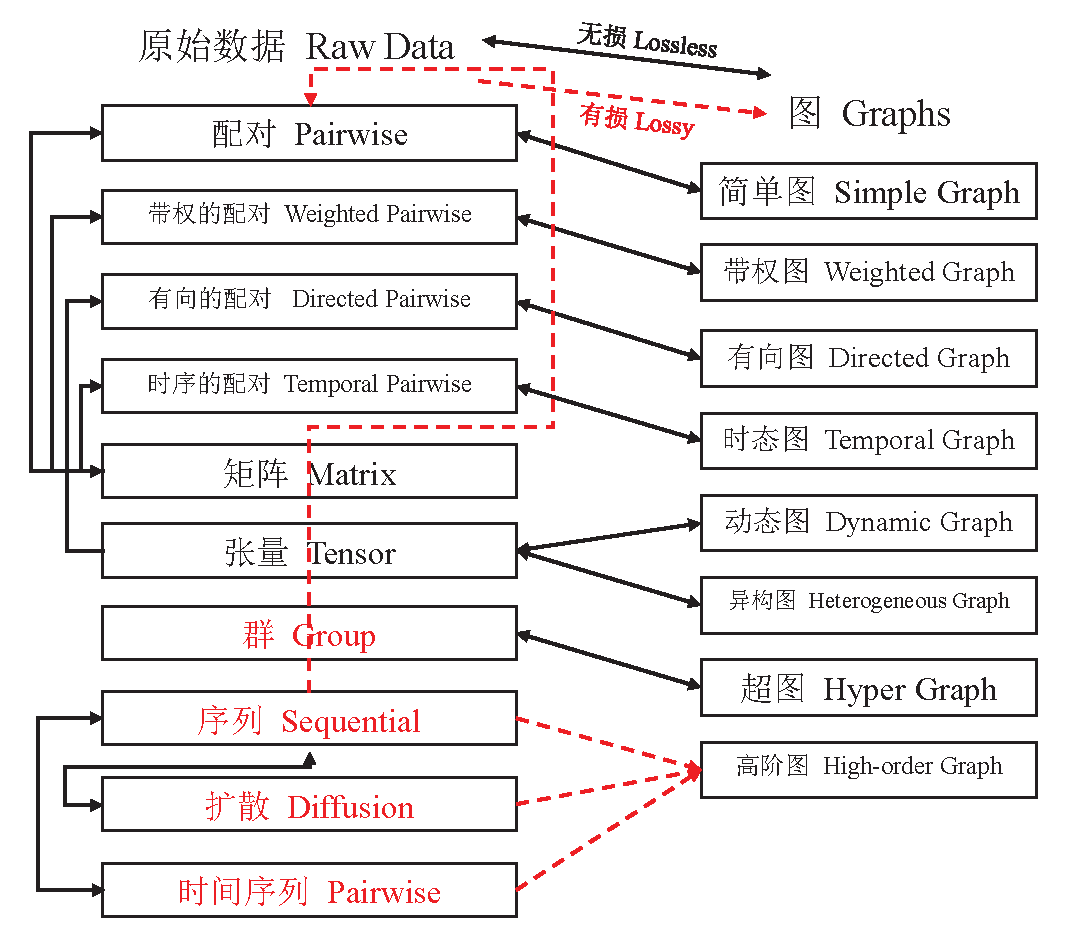
\includegraphics[scale=0.4]{pic/graphrep.eps}
		\column{0.4\textwidth}
		\begin{formal}
			图（graph）提供了一种通用的表示形式~\cite{ma2021graphdl}。
			\begin{itemize}
				\item 来自各个领域的许多系统的数据可以明确地被表示成图
				\item 许多其他类型的数据可以转换为图~\cite{xu2017networks}
			\end{itemize}
		\end{formal}
	\end{columns}
\end{frame}

\begin{frame}{将真实世界中的数据表示成图（续）}
	\begin{formal}
		大量的真实世界中的问题可以作为图上的一小组计算任务来解决。
		\begin{itemize}
			\item 节点为中心的任务（node-focused task）：\textbf{以节点为基本处理对象}，如{\color{red}节点分类（node classification）}（e.g. 异常节点检测~\cite{wen2024ta}、致病基因识别~\cite{saadat2024dna}）、{\color{red}链接预测（link prediction）}（e.g. 多药副作用预测~\cite{keshavarz2024pugnn}、药物-靶点亲和性预测~\cite{he2024drug}）
			\item 图为中心的任务（graph-focused task）：\textbf{以图为基本处理对象}，如{\color{red}图分类（graph classification）}（e.g. 分子活性预测~\cite{song2024mole}、楔形文字识别~\cite{stelzer2024cuneiform}）
		\end{itemize}
	\end{formal}
\end{frame}

\begin{frame}{真实世界中的图}
	\begin{figure}
		\label{fig:rw1-6}
		\centering
		\subfigure[事件图~\cite{xu2021event}]{
			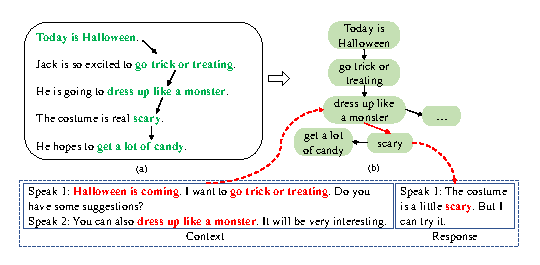
\includegraphics[width=0.22\textwidth]{pic/event.eps}		
		}
		\subfigure[计算机网络~\cite{nd2022}]{
			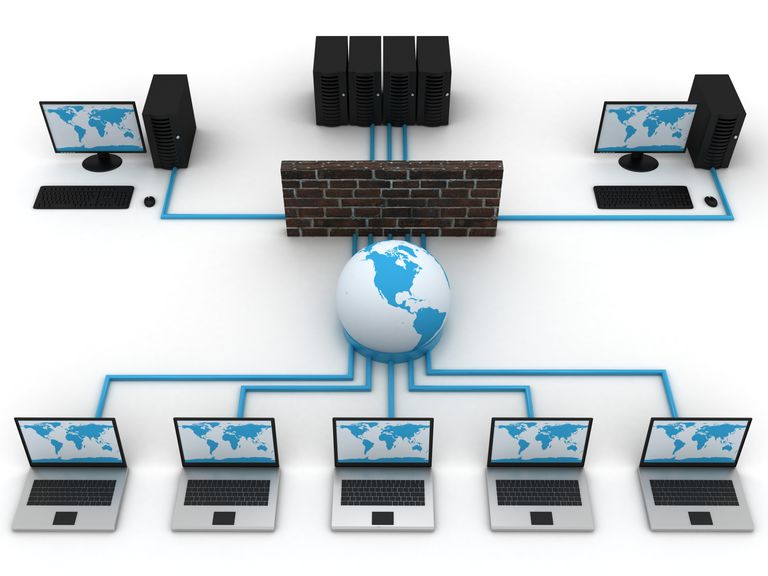
\includegraphics[width=0.22\textwidth]{pic/comnet.jpg}
		}
		\subfigure[疾病反应路径~\cite{agrawal2018pathway}]{
			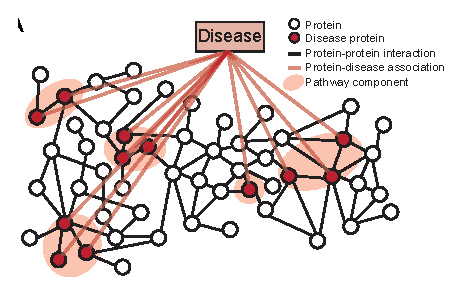
\includegraphics[width=0.2\textwidth]{pic/pathway.eps}
		}
		\subfigure[食物链~\cite{ator2007ecosystem}]{
			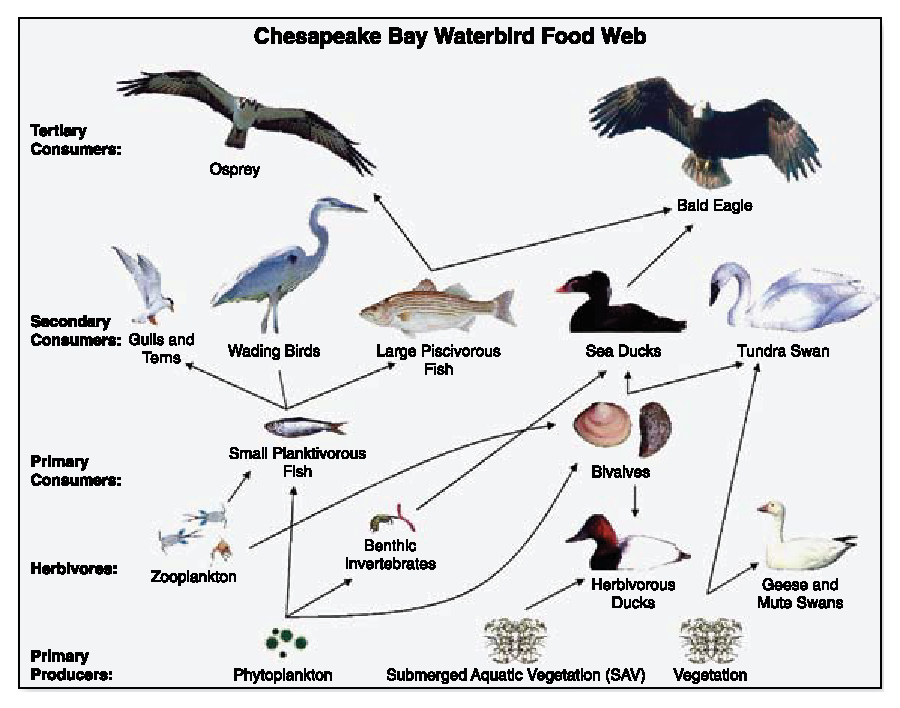
\includegraphics[width=0.2\textwidth]{pic/foodchain.eps}
		}
		\subfigure[粒子网络~\cite{koos2014particle}]{
			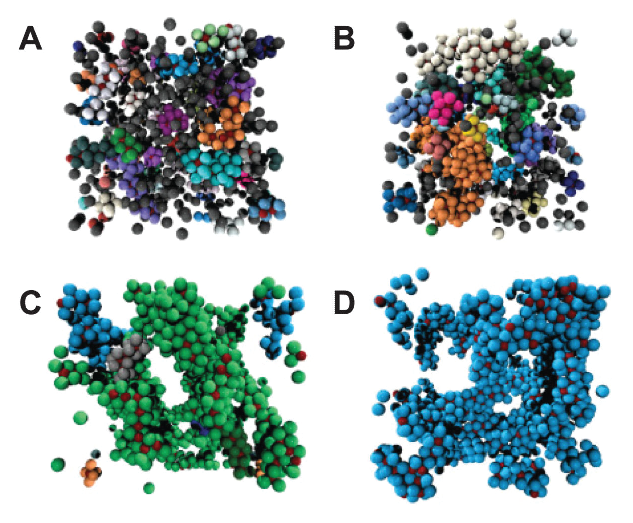
\includegraphics[width=0.2\textwidth]{pic/particle.eps}
		}
		\subfigure[地铁网络~\cite{crt2024}]{
			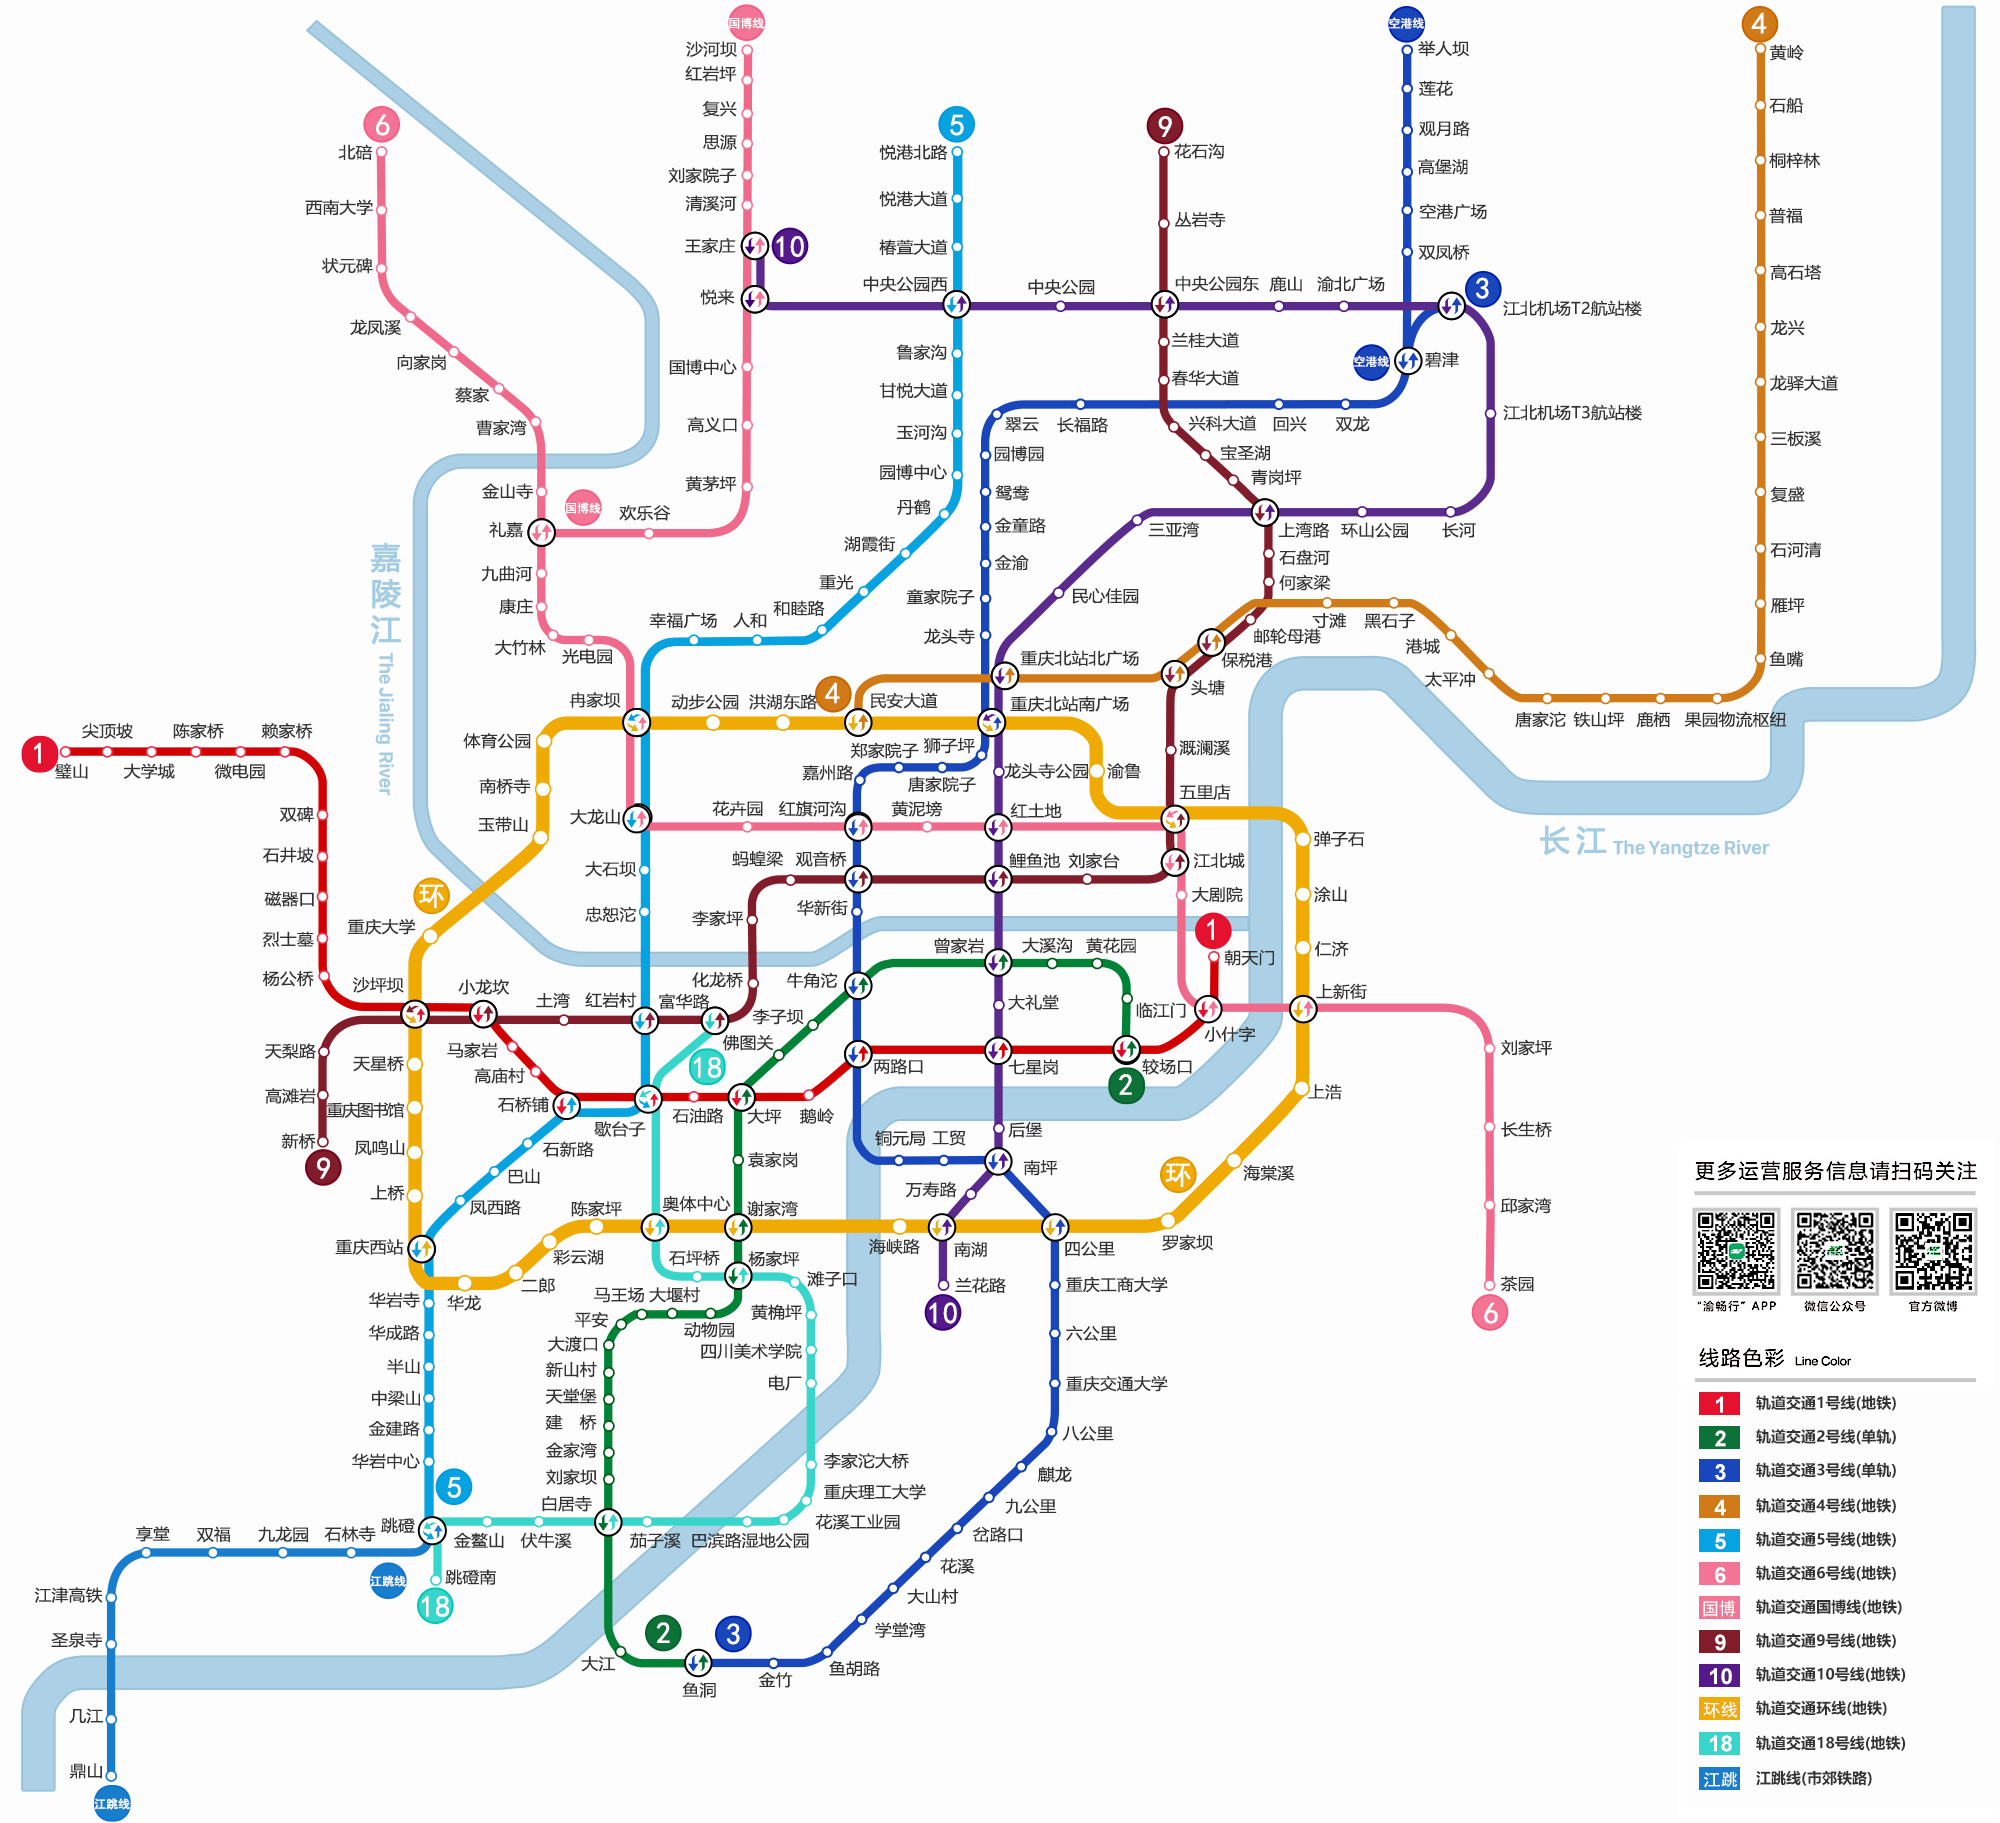
\includegraphics[width=0.2\textwidth]{pic/metro.png}
		}
	\end{figure}
\end{frame}

\begin{frame}{真实世界中的图（续）}
	\begin{figure}
		\label{fig:rw7-12}
		\centering
		\subfigure[社交网络~\cite{sn2022}]{
			
\includegraphics[width=0.2\textwidth]{pic/social.jpg}
		}
		\subfigure[经济网络~\cite{schweitzer2009economic}]{
			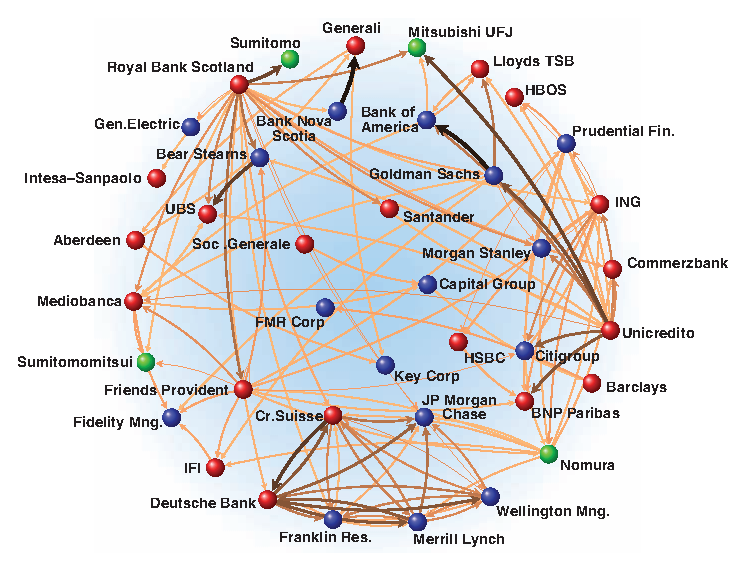
\includegraphics[width=0.2\textwidth]{pic/economic.eps}
		}
		\subfigure[通讯网络~\cite{cao2018airborne}]{
			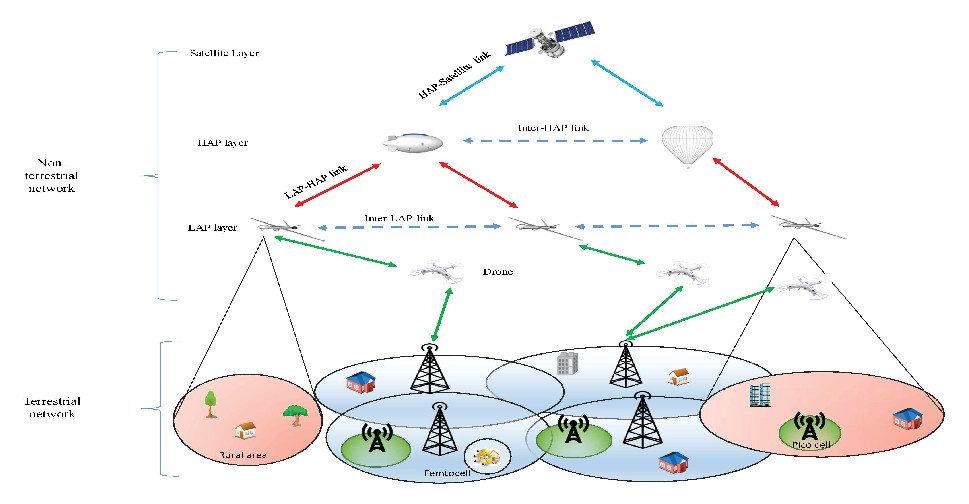
\includegraphics[width=0.2\textwidth]{pic/communi.eps}
		}
		\subfigure[引文网络~\cite{valtonen2022edu}]{
			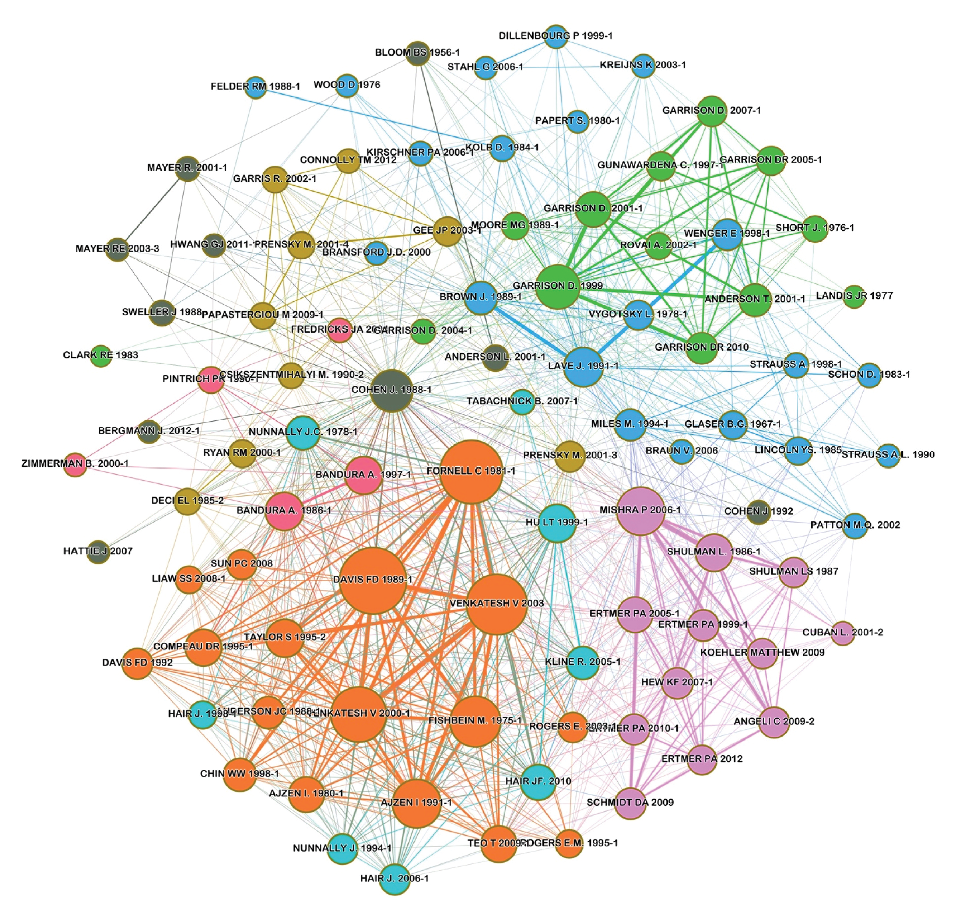
\includegraphics[width=0.2\textwidth]{pic/citation.eps}
		}
		\subfigure[互联网~\cite{mc2020web}]{
			
\includegraphics[width=0.2\textwidth]{pic/internet.jpg}
		}
		\subfigure[神经元网络~\cite{torres2022mind}]{
			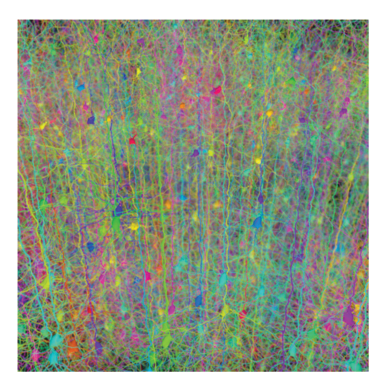
\includegraphics[width=0.2\textwidth]{pic/neuron.eps}
		}
	\end{figure}
\end{frame}

\begin{frame}{真实世界中的图（续）}
	\begin{figure}
		\label{fig:rw13-18}
		\centering
		\subfigure[知识图谱~\cite{nickel2015know}]{
			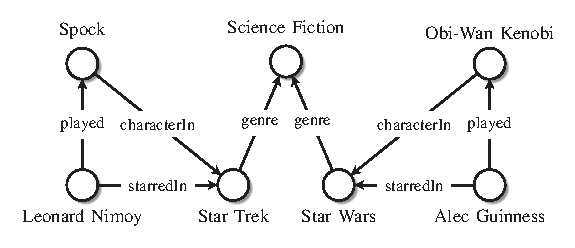
\includegraphics[width=0.2\textwidth]{pic/knowledge.eps}
		}
		\subfigure[基因调控网络~\cite{mcdunn3illness}]{
			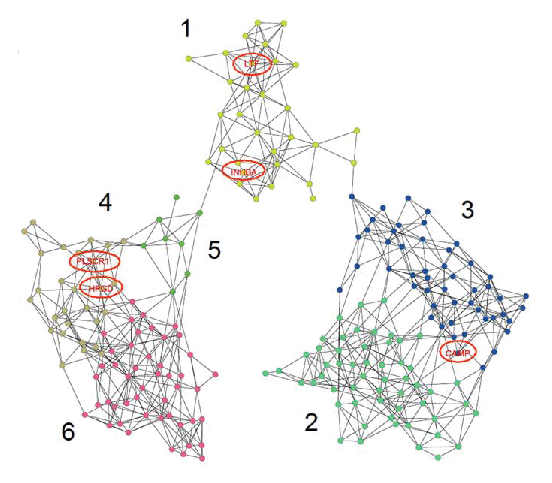
\includegraphics[width=0.2\textwidth]{pic/regulatory.eps}
		}
		\subfigure[场景图~\cite{eck2023graphics}]{
			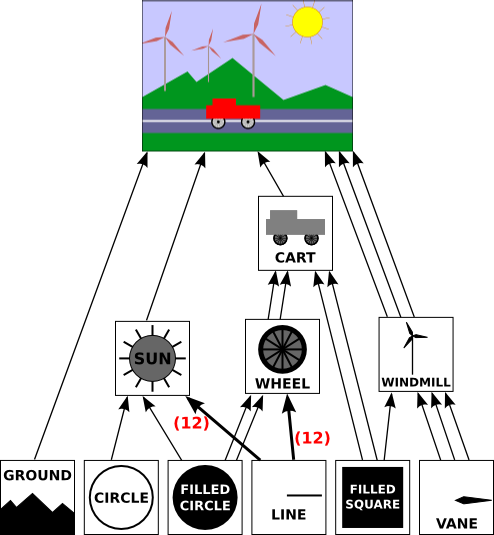
\includegraphics[width=0.2\textwidth]{pic/scene.png}
		}
		\subfigure[代码图~\cite{bond2010breadcrumbs}]{
			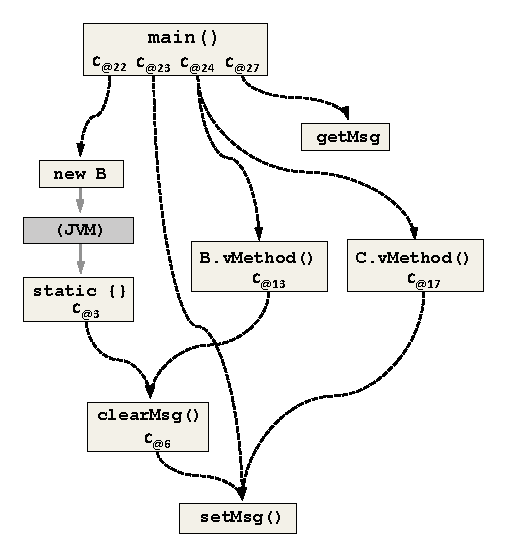
\includegraphics[width=0.15\textwidth]{pic/code.eps}
		}
		\subfigure[分子~\cite{chen2021chemical}]{
			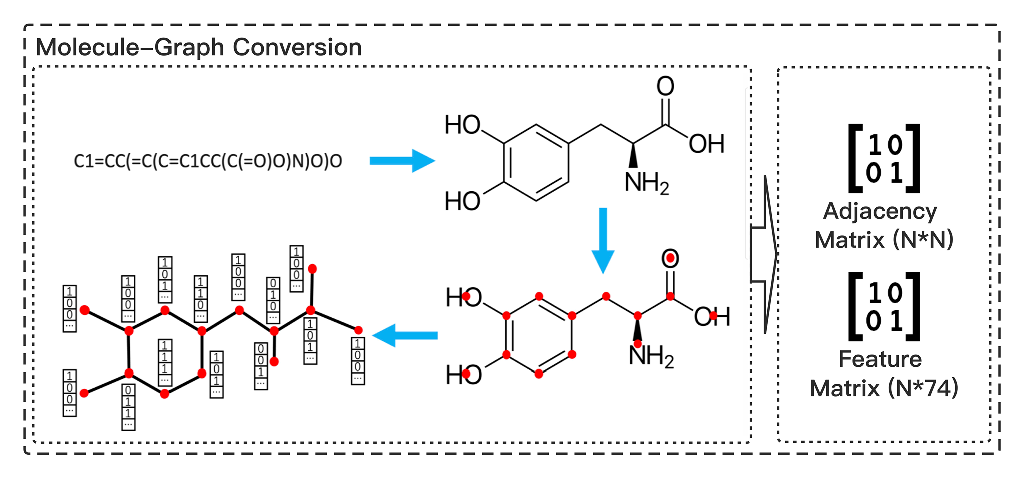
\includegraphics[width=0.2\textwidth]{pic/molecule.eps}
		}
		\subfigure[3D形状~\cite{wiki2023dolphin}]{
			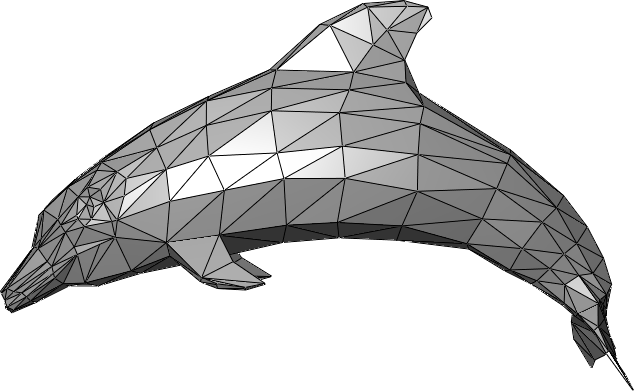
\includegraphics[width=0.2\textwidth]{pic/3dshape.png}
		}
	\end{figure}
\end{frame}

\begin{frame}{为什么经典的卷积神经网络不能胜任图上的计算任务？}
	\begin{figure}
		\centering
		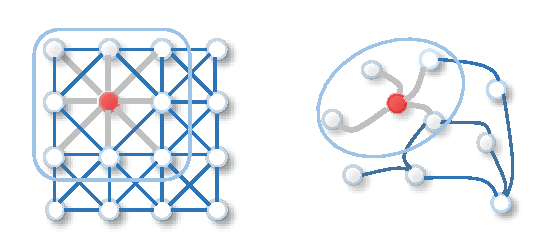
\includegraphics[scale=0.6]{pic/cnngnn.eps}
	\end{figure}
	\begin{itemize}
		\item \textbf{二维卷积} \\
		图像中的每个像素（pixel）被视为一个节点，邻居大小由滤波器决定。二维卷积取目标节点的{\color{red}有序、固定数量}的邻居节点的像素值进行加权平均。
		\item \textbf{图卷积} \\
		图卷积运算的比较简单的方案也是对邻居节点进行加权平均，但是与二位图像数据不同，\textbf{目标节点的邻居节点是无序的且不同目标节点的邻居数量不一}。
	\end{itemize}
\end{frame}

\begin{frame}{最初代的图神经网络}
	\begin{itemize}
		\item 2005年，Marco Gori、Gabriele Monfardini和Franco Scarselli最早提出图神经网络（graph neural network，GNN）~\cite{gori2005gnn}的概念。在此之前，处理图数据的方法是在数据的预处理阶段将图转换为用一组向量表示。
		\item 2009年，Franco Scarselli博士在其论文~\cite{scarselli2008gnn}中定义了图神经网络的理论基础，并做了一定程度的改进。早期阶段的GNN主要是以RNN为主体框架，通过简单的特征映射和节点聚集为每个节点生成向量式表达，不能很好地应对现实中复杂多变的图数据。
		\item 针对此情况，Yann LeCun的学生Joan Bruna等人提出将CNN应用到图上，通过对卷积算子巧妙的转换，提出了基于频域和基于空域的图卷积网络，并衍生了许多变体。
	\end{itemize}
\end{frame}

\begin{frame}{频域上的图卷积}
	图上基于频域（spectral-based）的卷积定义为图信号（graph signal）$x\in\mathbb{R}^N$和傅里叶域（Fourier domain）上的滤波器$g_\theta=\text{diag}\left(\theta\right)$（$\theta\in\mathbb{R}^N$为参数）
	\begin{equation}
		g_\theta\star x=Ug_\theta U^\top x,
	\end{equation}
	$U$为对称归一化拉普拉斯矩阵$L=I_N-D^{-\frac{1}{2}}AD^{-\frac{1}{2}}=U\Lambda U^\top$的特征向量，$\Lambda$为特征值组成的对角阵，$U^\top x$为$x$的图傅里叶变换（graph Fourier transform）。$g_\theta$是$L$的特征值的函数，记作$g_\theta\left(\Lambda\right)$。为节约运算开销，使用$K$阶切比雪夫多项式（Chebyshev polynomials）$T_k\left(x\right)$拟合$g_\theta\left(\Lambda\right)$
	\begin{equation}
		g_{\theta^\prime}\left(\Lambda\right)\approx\sum\limits_{k=0}^K\theta^\prime_k T_k\left(\tilde\Lambda\right),
	\end{equation}
	$\tilde\Lambda=\frac{2}{\lambda_{\text{max}}}\lambda-I_N$（$\lambda_{\text{max}}$为$L$的最大特征值），$\theta^\prime \in\mathbb{R}^K$是切比雪夫多项式的系数向量。
\end{frame}

\begin{frame}{频域上的图卷积（续）}
	切比雪夫多项式定义为$T_k\left(x\right)=2xT_{k-1}\left(x\right)-T_{k-2}\left(x\right)\,\text{with}\,T_0\left(x\right)=1\,\text{and}T_1\left(x\right)=x$。从而
	\begin{equation}
		g_\theta\star x\approx\sum\limits_{k=0}^K\theta^\prime_kT_k\left(\tilde{L}\right),
	\end{equation}
	$\tilde{L}=\frac{2}{\lambda_{\text{max}}}L-I_N$，因为有$\left(U\Lambda U^\top\right)^k=U\Lambda^kU^\top$。注意到，前一个表达式计算的是拉普拉斯矩阵的K阶多项式，刻画了节点的K跳邻居。
\end{frame}

\begin{frame}{频域转向空域}
	近似取$\Lambda_{\text{max}}\approx2$，
	\begin{equation}
		g_\theta\star x\approx\theta^\prime_0x+\theta^\prime_1\left(L-I_N\right)x=\theta^\prime_0x-\theta^\prime_1D^{-\frac{1}{2}}AD^{-\frac{1}{2}}x,
	\end{equation}
	$\theta^\prime_0$和$\theta^\prime_1$是两个自由的参数。然后，连续应用这种形式的过滤器可以有效地卷积节点的K阶邻域，其中K可以是神经网络模型中连续滤波操作或卷积层的数量。
	实际运算时，压缩参数有利于避免过拟合和降低运算负载，
	\begin{equation}
		g_\theta\star x\approx\theta\left(I_N+D^{-\frac{1}{2}}AD^{-\frac{1}{2}}\right)x,
	\end{equation}
	$\theta=\theta^\prime_0=-\theta^\prime_1$。由于$I_N+D^{-\frac{1}{2}}AD^{-\frac{1}{2}}$的特征值落在$\left[0,2\right]$。因此，在深度神经网络模型中重复应用该运算符可能会导致数值不稳定和梯度消失。
\end{frame}



\section{图卷积神经网络（GCN）}



\begin{frame}{逐层传播规则}
	\begin{formal}
		在论文~\cite{kipf2017gcn}中，图卷积神经网络（graph convolutional network，GCN）的逐层传播规则（layer-wise propagation rule）定义如下：
		\begin{equation}
			\label{eq:gcnlp}
			\textbf{H}^{\left(\ell+1\right)}=\sigma\left(\tilde{\textbf{D}}^{-\frac{1}{2}}\tilde{\textbf{A}}\tilde{\textbf{D}}^{-\frac{1}{2}}\textbf{H}^{\left(\ell\right)}\textbf{W}^{\left(\ell\right)}\right),
		\end{equation}
		其中，$\sigma$为激活函数（通常为ReLU函数），$\textbf{H}^{\left(\ell\right)}$、$\textbf{W}^{\left(\ell\right)}$为节点特征矩阵和参数矩阵，$\tilde{\textbf{A}}=\textbf{A}+\textbf{I}_{\left|\mathscr{V}\right|}$（其中$\textbf{I}_{\left|\mathscr{V}\right|}$为大小为节点个数的单位对角阵），$\tilde{\textbf{D}}$为新邻接矩阵$\tilde{\textbf{A}}$对应的度矩阵。
	\end{formal}
\end{frame}

\begin{frame}{GCN节点分类——输入图）}
	\begin{figure}
		\centering
		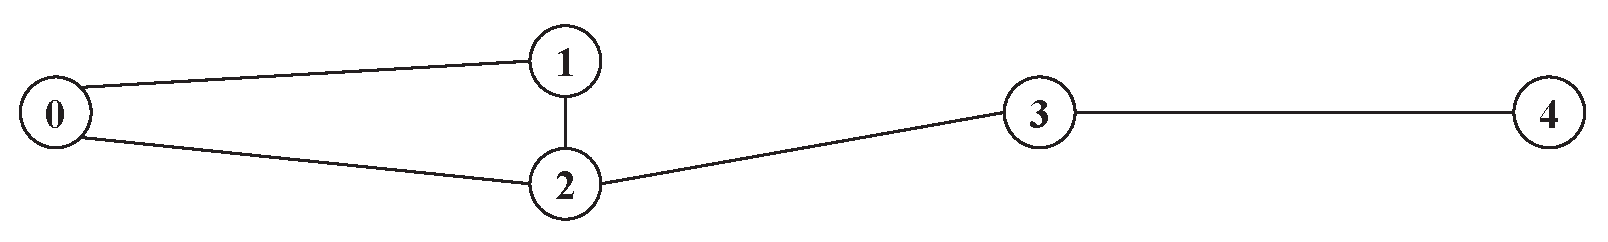
\includegraphics[scale=0.3]{pic/graph.eps}
	\end{figure}
	\begin{equation}
		\setlength{\arraycolsep}{2pt}
		\begin{matrix}
			\textbf{A}=\begin{bmatrix}
				0 & 1 & 1 & 0 & 0 \\
				1 & 0 & 1 & 0 & 0 \\
				1 & 1 & 0 & 1 & 0 \\
				0 & 0 & 1 & 0 & 1 \\
				0 & 0 & 0 & 1 & 0
			\end{bmatrix} &
			\textbf{H}^{\left(0\right)}=\begin{bmatrix} 
				-1.5 & 0.5 \\
				-0.5 & 1.0 \\
				-0.5 & 0 \\
				1.0 & 0.6 \\
				1.6 & -0.4
			\end{bmatrix}
		\end{matrix}
	\end{equation}
	\begin{equation}
		\setlength{\arraycolsep}{2pt}
		\widehat{\textbf{A}}=\tilde{\textbf{D}}^{-\frac{1}{2}}\tilde{\textbf{A}}\tilde{\textbf{D}}^{-\frac{1}{2}}=\begin{bmatrix}
			0.3333 & 0.3333 & 0.2887 & 0 & 0 \\
			0.3333 & 0.3333 & 0.2887 & 0 & 0 \\
			0.2887 & 0.2887 & 0.2500 & 0.2887 & 0 \\
			0 & 0 & 0.2887 & 0.3333 & 0.4082 \\
			0 & 0 & 0 & 0.4082 & 0.5000
		\end{bmatrix}
	\end{equation}
\end{frame}

\begin{frame}{GCN节点分类——前向传播（第1层卷积）}
	\begin{figure}
		\centering
		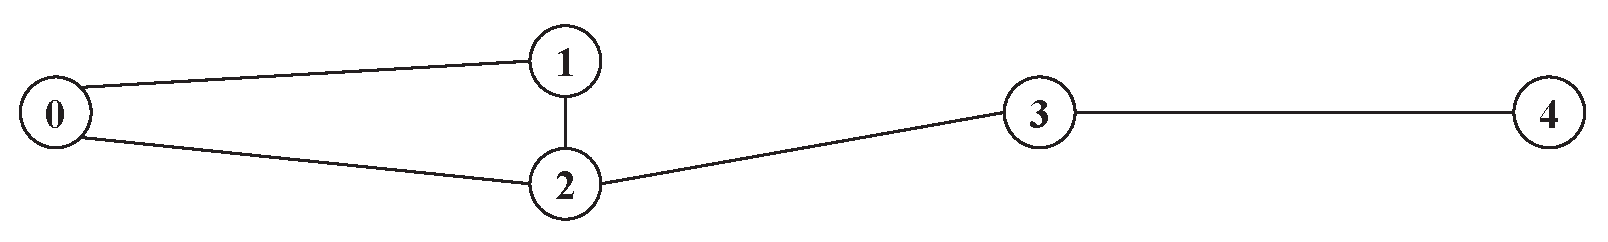
\includegraphics[scale=0.3]{pic/graph.eps}
	\end{figure}
	\begin{equation}
		\setlength{\arraycolsep}{2pt}
		\textbf{W}^{\left(0\right)}=\begin{bmatrix}
			1.4897 & 1.4172 & -1.2075 & 1.6302\\
			1.4090 & 0.6715 & 0.7172 & 0.4889
		\end{bmatrix}
	\end{equation}
	\begin{equation}                      
		\setlength{\arraycolsep}{2pt}
		\textbf{H}^{\left(1\right)}=\sigma\left(\widehat{\textbf{A}}\textbf{H}^{\left(0\right)}\textbf{W}^{\left(0\right)}\right)=\begin{bmatrix}
			0 & 0 & 1.3379 & 0 \\
			0 & 0 & 0.3907 & 0 \\
			0.2379 & 0 & 0.9343 & 0 \\
			1.3063 & 1.2182 & 0 & 1.3909 \\
			1.8633 & 1.7425 & 0 & 1.9917
		\end{bmatrix}
	\end{equation}
\end{frame}

\begin{frame}{GCN节点分类——前向传播（第2层卷积）}
	\begin{figure}
		\centering
		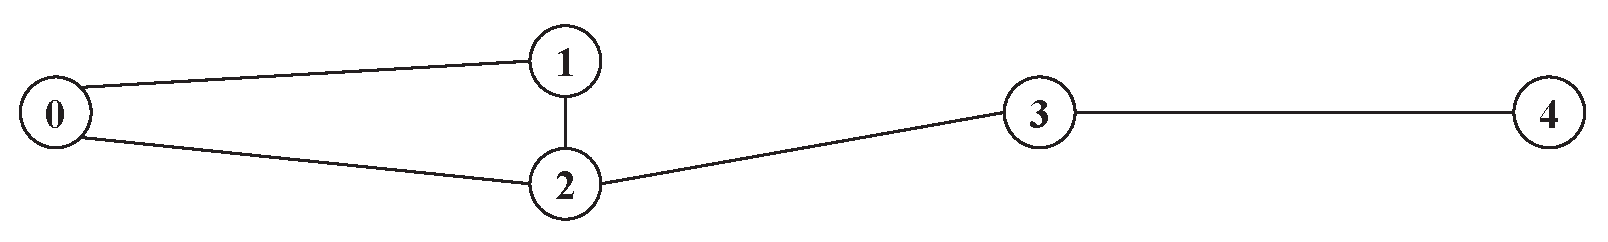
\includegraphics[scale=0.3]{pic/graph.eps}
	\end{figure}
	\begin{equation}
		\setlength{\arraycolsep}{2pt}
		\textbf{W}^{\left(1\right)}=\begin{bmatrix}
			1.0347 & -0.7873 \\
			0.7269 & 0.8884 \\
			-0.3034 & -1.1471 \\
			0.2939 & -1.0689
		\end{bmatrix}
	\end{equation}
	\begin{equation}
		\setlength{\arraycolsep}{2pt}
		\textbf{H}^{\left(2\right)}=\sigma\left(\widehat{\textbf{A}}\textbf{H}^{\left(1\right)}\textbf{W}^{\left(1\right)}\right)=\begin{bmatrix}
			0 & 0\\
			0 & 0\\
			0.5201 & 0\\
			2.4143 & 0\\
			2.9701 & 0
		\end{bmatrix}
	\end{equation}
\end{frame}

\begin{frame}{GCN用于节点分类——计算概率}
	\begin{figure}
		\centering
		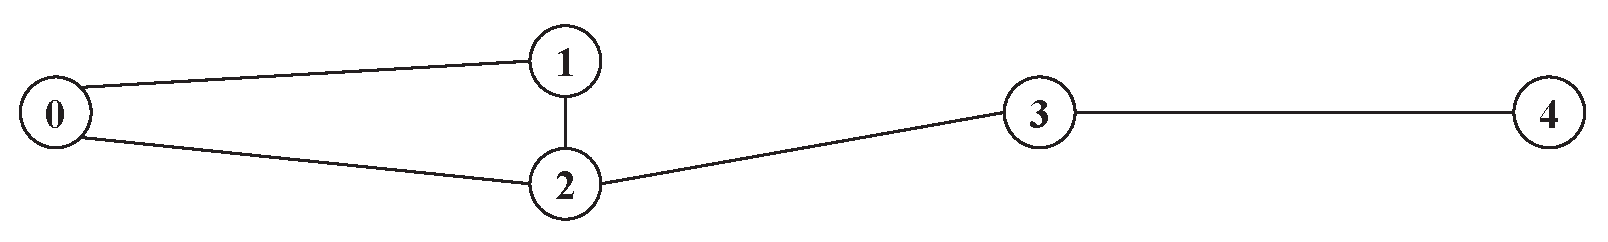
\includegraphics[scale=0.3]{pic/graph.eps}
	\end{figure}
	\begin{equation}
		\text{Softmax}\left(\textbf{H}^{\left(2\right)}\right)=\frac{\exp\left(\textbf{H}^{\left(2\right)}_i\left[j\right]\right)}{\sum\limits_{k=0}^1\textbf{H}^{\left(2\right)}_i\left[k\right]}\,\,\text{for}\,\,\begin{matrix}
			j\gets0\,\text{to}\,1 \\
			i\gets0\,\text{to}\,4
		\end{matrix}
	\end{equation}
	最后一层（第2层）卷积输出的节点特征矩阵经过Softmax归一化后，得到每个节点隶属于不同类别的{\color{red}概率}：
	\begin{equation}
		\textbf{P}=\begin{bmatrix}
			0.5000 & 0.5000 \\
			0.5000 & 0.5000 \\
			0.6272 & 0.3728 \\
			0.9179 & 0.0821 \\
			0.9512 & 0.0488
		\end{bmatrix}
	\end{equation}
\end{frame}

\begin{frame}{GCN用于节点分类——计算损失}
	\begin{figure}
		\centering
		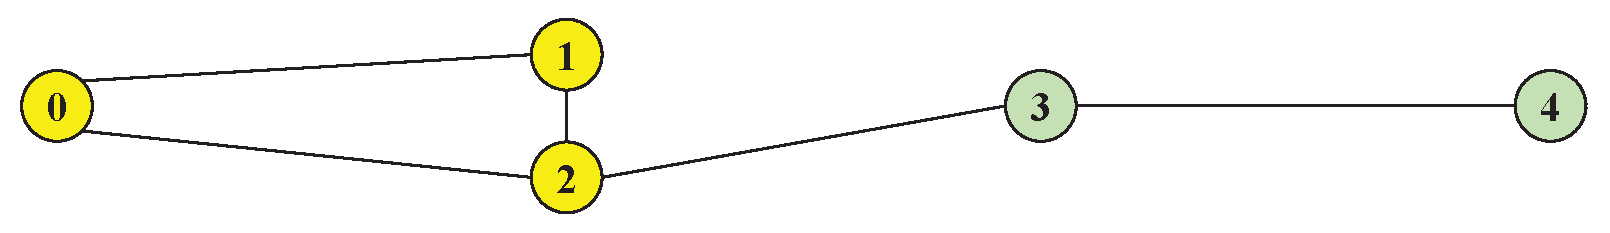
\includegraphics[scale=0.3]{pic/labeledgraph.eps}
	\end{figure}
	节点标签
	\begin{equation}
		\vec{\textbf{l}}=\left[0,0,0,1,1\right]
	\end{equation}
	分类问题的损失由交叉熵（cross entropy）损失函数计算：
	\begin{equation}
		\begin{aligned}
			\mathcal{L}&=-\frac{1}{N}\sum\limits_{i=1}^{N}\left(y_i\log p\left(\hat{y}_i\right)+\left(1-y_i\right)\log p\left(1-\hat{y}_i\right)\right)\\
			&=-\frac{1}{5}\sum\limits_{i=0}^4\ln\left(\textbf{P}\left[i,\vec{\textbf{l}}\left[i\right]\right]\right)\approx1.4745
		\end{aligned}
	\end{equation}
\end{frame}

\begin{frame}{逐层传播规则不是一成不变的！}
	\begin{formal}
		\begin{itemize}
			\item {\color{red}\textbf{有向图}} \\
			考虑{\color{red}有向图的入度、出度矩阵的不一致}，Stefan Drenbach最先给出了GCN的有向适应（directed adaptation）~\cite{dernbach2018directed}。\\
			{\color{red}库函数GCN实现}中的处理方法为：
			\begin{equation}
				\textbf{H}^{\left(\ell+1\right)}=\sigma\left(\tilde{\textbf{D}}_{in}^{-\frac{1}{2}}\tilde{\textbf{A}}\tilde{\textbf{D}}_{out}^{-\frac{1}{2}}\textbf{H}^{\left(\ell\right)}\textbf{W}^{\left(\ell\right)}\right)
			\end{equation}
		\end{itemize}
	\end{formal}
\end{frame}

\begin{frame}{逐层传播规则不是一成不变的！（续）}
	\begin{formal}
		\begin{itemize}
			\item {\color{red}\textbf{自环}} \\
			在公式\ref{eq:gcnlp}中，$\tilde{\textbf{A}}=\textbf{A}+\textbf{I}_{\left|\mathscr{V}\right|}$，即给每个节点自身到自身连接了一条边。由于图的拓扑结构（尤指环状结构（circles）），节点A传递给其他节点的信息可能会再次回到自身。论文\cite{lampert2023loop}中甚至还证明在某些数据集上，添加自环反而会破坏节点对自身特征信息的保留。
			\item {\color{red}\textbf{拉普拉斯矩阵的归一化}} \\
			标准GCN中的拉普拉斯矩阵$\textbf{L}=\tilde{\textbf{D}}^{-\frac{1}{2}}\tilde{\textbf{A}}\tilde{\textbf{D}}^{-\frac{1}{2}}$采用了对称归一化方法，也可采用左归一化、右归一化和不采用归一化。
		\end{itemize}
	\end{formal}
\end{frame}

\begin{frame}{消息传递形式}
	论文\cite{kipf2017gcn}中还给出了节点视角的逐层传播公式：
	\begin{equation}
		\label{eq:gcnmicro}
		\begin{aligned}
			\vec{\textbf{h}}_i^{\left(\ell+1\right)}&=\sigma\left(\sum\limits_{j\in\mathcal{N}\left(i\right)}\frac{1}{c_{ij}}\vec{\textbf{h}}_j^{\left(\ell\right)}\textbf{W}^{\left(\ell\right)}\right), \\
			c_{ij}&=\sqrt{\tilde{\textbf{D}}_{ii}\tilde{\textbf{D}}_{jj}},
		\end{aligned}
	\end{equation}
	其中，$\vec{\textbf{h}}_i^{\left(\ell+1\right)}$为节点$i$在第$\ell+1$层的节点特征行向量。
	
	回顾整张图上的逐层传播规则（公式\ref{eq:gcnlp}），
	\begin{equation*}
		\textbf{H}^{\left(\ell+1\right)}=\sigma\left(\tilde{\textbf{D}}^{-\frac{1}{2}}\tilde{\textbf{A}}\tilde{\textbf{D}}^{-\frac{1}{2}}\textbf{H}^{\left(\ell\right)}\textbf{W}^{\left(\ell\right)}\right).
	\end{equation*}
\end{frame}

\begin{frame}{消息传递形式（续）}
	将公式\ref{eq:gcnlp}中的矩阵-矩阵乘法/矩阵-向量乘法分块写出：
	\begin{equation}
		\setlength{\arraycolsep}{2pt}
		\begin{bmatrix}
			\vdots \\
			\vec{\textbf{h}}_i^{\left(\ell+1\right)} \\
			\vec{\textbf{h}}_j^{\left(\ell+1\right)} \\
			\vdots
		\end{bmatrix}
		=\begin{bmatrix}
			\ddots &  &  & \\
			& \tilde{\textbf{D}}_{ii}^{-\frac{1}{2}} &  & \\
			&  & \tilde{\textbf{D}}_{jj}^{-\frac{1}{2}} & \\
			&  &  & \ddots
		\end{bmatrix}
		\begin{bmatrix}
			\vdots & \vdots & \vdots & \vdots \\
			\vdots & 1 & 1 & \vdots \\
			\vdots & 1 & 1 & \vdots\\
			\vdots & \vdots & \vdots & \vdots
		\end{bmatrix}
		\begin{bmatrix}
			\ddots &  &  & \\
			& \tilde{\textbf{D}}_{ii}^{-\frac{1}{2}} &  & \\
			&  & \tilde{\textbf{D}}_{jj}^{-\frac{1}{2}} & \\
			&  &  & \ddots
		\end{bmatrix}
		\begin{bmatrix}
			\vdots \\
			\vec{\textbf{h}}_i^{\left(\ell\right)} \\
			\vec{\textbf{h}}_j^{\left(\ell\right)} \\
			\vdots
		\end{bmatrix}
	\end{equation}
	显然，{\color{red}公式\ref{eq:gcnlp}和公式\ref{eq:gcnmicro}在形式上一致}。
\end{frame}

\begin{frame}{消息传递形式（续）}
	\begin{figure}
		\centering
		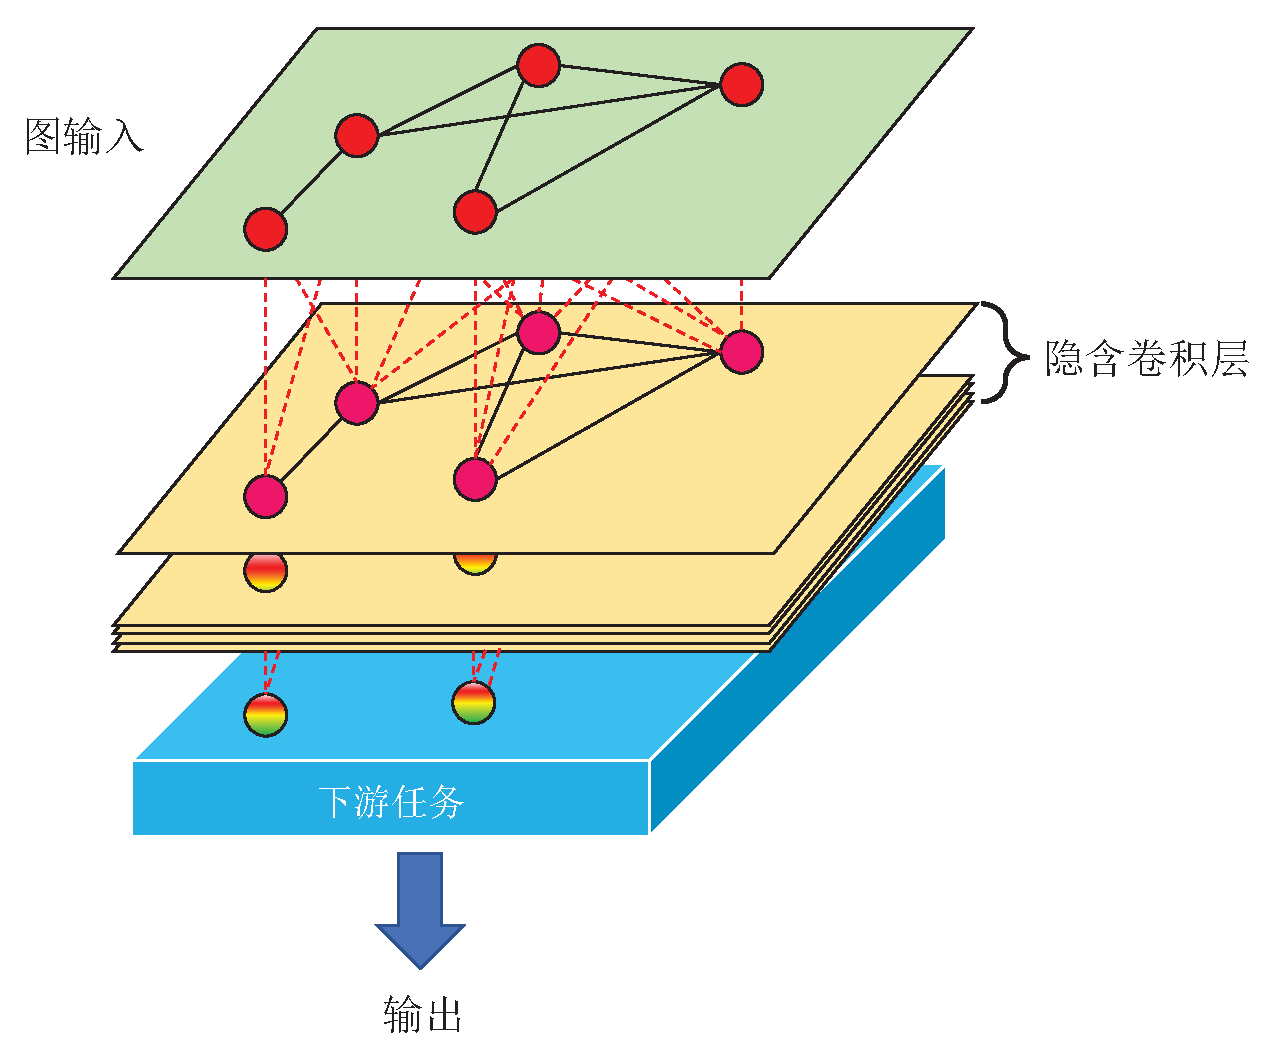
\includegraphics[scale=0.4]{pic/gcn.eps}
	\end{figure}
\end{frame}

\begin{frame}{主流图神经网络Python库}
	\begin{figure}
		\begin{center}
			
\includegraphics[scale=0.03]{pic/dgl.png}\quad\quad\quad
			
\includegraphics[scale=0.12]{pic/pyg.png}
		\end{center}
	\end{figure}
	Deep graph library（DGL）~\cite{wang2019dgl}\cite{dgl2024}和PyTorch Geometric（PyG）~\cite{fey2019pyg}\cite{pyg2024}都集成了：
	\begin{itemize}
		\item 不同类型图的存储对象
		\item 主流图结构化数据集
		\item 图神经网络模型（{\color{red}大部分是2020年及以前}）
		\item CPU、CPU+GPU、GPU、TPU等计算平台的访存计算优化策略
		\item 后端接口：PyTorch (DGL \& PyG), TensorFlow (DGL), MXNet (DGL)
	\end{itemize}
\end{frame}



\section{图采样和聚合（GraphSAGE）}



\begin{frame}{算法基本流程}
	\begin{algorithm}[H]
		\label{algo:sage}
		\caption{\footnotesize GraphSAGE生成节点的嵌入表示（embeddings）~\cite{hamilton2017graphsage}}
		\LinesNumbered
		\KwIn{图$\mathscr{G}\left(\mathscr{V},\mathscr{E}\right)$，初始节点特征$\textbf{H}^{\left(0\right)}=\left[\vec{\textbf{h}^{\left(0\right)}_0}^\top\dots\vec{\textbf{h}^{\left(0\right)}_{\left|\mathscr{V}\right|}}^\top\right]^\top$}
		\KwOut{最终节点特征 $\textbf{H}^{\left(L\right)}$}
		\For{$\ell=0\dots L-1$}{
			\For{$i\in\mathscr{V}$}{
				$\vec{\textbf{h}}^{\left(\ell\right)}_{\mathcal{N}\left(i\right)}\gets\text{AGGREGATE}\left\{\vec{\textbf{h}}^{\left(\ell\right)}_j,\,\,\forall j\in\mathcal{N}\left(i\right)\right\}$\;
				$\vec{\textbf{h}}^{\left(\ell+1\right)}_i\gets\sigma\left(\text{COMBINE}\left(\vec{\textbf{h}}^{\left(\ell\right)}_i,\vec{\textbf{h}}^{\left(\ell\right)}_{\mathcal{N}\left(i\right)}\right)\cdot\textbf{W}^{\left(\ell\right)}\right)$\;
			}
			$\vec{\textbf{h}}^{\left(\ell+1\right)}_k\gets\vec{\textbf{h}}^{\left(\ell+1\right)}_k/\|\vec{\textbf{h}}^{\left(\ell+1\right)}_k\|_2,\,\,\forall k\in\mathscr{V}$\;
		}
	\end{algorithm}
\end{frame}

\begin{frame}{聚合函数（AGGREGATE）}
	\begin{itemize}
		\item {\color{red}最大值/最小值/均值聚合函数（max/min/mean aggregator）}
		\begin{equation}
			\vec{\textbf{h}}^{\left(\ell+1\right)}_i=\sigma\left(\text{MAX/MIN/MEAN}\left(\left\{\vec{\textbf{h}}^{\left(\ell\right)}_i\right\},\left\{\vec{\textbf{h}}^{\left(\ell+1\right)}_j,\,\forall\, j\in\mathcal{N}\left(i\right)\right\}\right)\textbf{W}^{\left(\ell\right)}\right)
		\end{equation}
		\item {\color{red}LSTM聚合函数}\\
		由于输入是顺序的，LSTM不是置换不变的（permutation invariant）。需要将LSTM应用于节点邻居的随机置换（random permutation）使得LSTM能在无序集上进行操作~\cite{hamilton2017graphsage}。
		\item {\color{red}Pool聚合函数}\\
		\begin{equation}
			\text{AGGREGATE}_k^{pool}=\max\left(\left\{\sigma\left(\vec{\textbf{h}}^{\left(\ell\right)}_j\textbf{W}^{\left(\ell\right)}\right),\,\forall\, j\in\mathcal{N}\left(i\right)\right\}\right)
		\end{equation}
	\end{itemize}
\end{frame}

\begin{frame}{归纳式学习vs转导式学习}
	\begin{formal}
		\begin{itemize}
			\item {\color{red}\textbf{归纳式学习（inductive learning）}} \\
			从观察到的训练案例推理出一般规则，然后将其应用于测试案例。\\
			根据已有的标记训练数据集构建和训练模型，然后使用这个模型应用在从未遇到过的测试数据集。
			\item {\color{red}\textbf{转导式学习（transductive learning）}} \\
			从观察到的特定（训练）案例推理到特定（测试）案例。\\
			与归纳式学习相比，转导式学习技术事先观察了所有数据，包括训练和测试数据集。从已经观察到的训练数据集中学习，然后预测测试数据集的标签。即使不知道测试数据集的标签，也可以在学习过程中利用这些数据中存在的模式和其他信息~\cite{vm2020intr}。
		\end{itemize}
	\end{formal}
\end{frame}

\begin{frame}{GraphSAGE链接预测——输入图}
	\begin{figure}
		\centering
		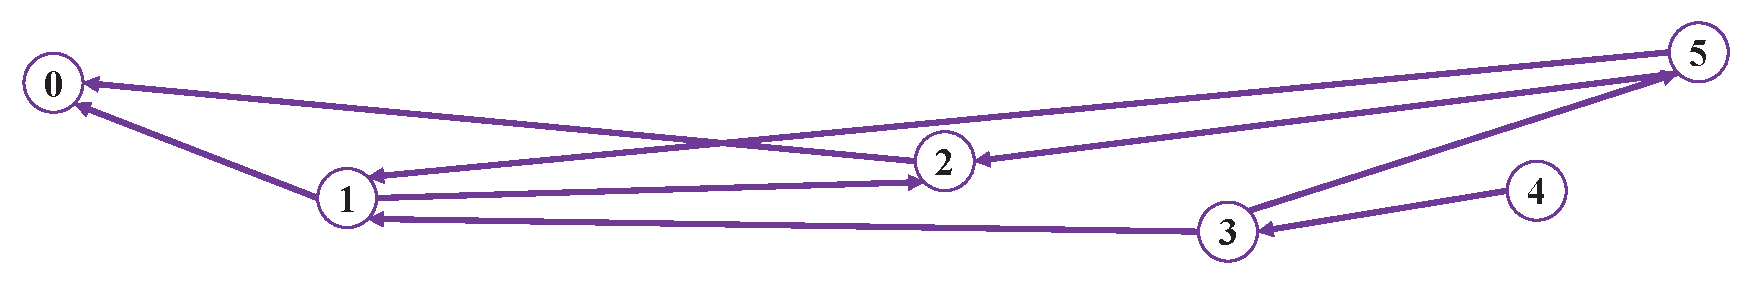
\includegraphics[scale=0.4]{pic/graph2.eps}
	\end{figure}
	\begin{equation}
		\setlength{\arraycolsep}{2pt}
		\begin{matrix}
		\textbf{A}=\begin{bmatrix}
			0 & 0 & 0 & 0 & 0 & 0\\
			1 & 0 & 1 & 0 & 0 & 0 \\
			1 & 0 & 0 & 0 & 0 & 0 \\
			0 & 1 & 0 & 0 & 0 & 1 \\
			0 & 0 & 0 & 1 & 0 & 0 \\
			0 & 1 & 1 & 0 & 0 & 0
		\end{bmatrix} &
		\textbf{H}^{\left(0\right)}=\begin{bmatrix}
			\vec{\textbf{h}}^{\left(0\right)}_0\\
			\vec{\textbf{h}}^{\left(0\right)}_1 \\
			\vec{\textbf{h}}^{\left(0\right)}_2 \\
			\vec{\textbf{h}}^{\left(0\right)}_3 \\
			\vec{\textbf{h}}^{\left(0\right)}_4 \\
			\vec{\textbf{h}}^{\left(0\right)}_5
		\end{bmatrix}
		=\begin{bmatrix}
			-1.5 & 2.0 \\
			-0.5 & 1.3 \\
			2.0 & 1.5 \\
			1.7 & 2.2 \\
			1.4 & -0.1 \\
			0.8 & -0.9
		\end{bmatrix}
		\end{matrix}
	\end{equation}
\end{frame}

\begin{frame}{GraphSAGE用于链接预测——前向传播}
	\begin{figure}
		\centering
		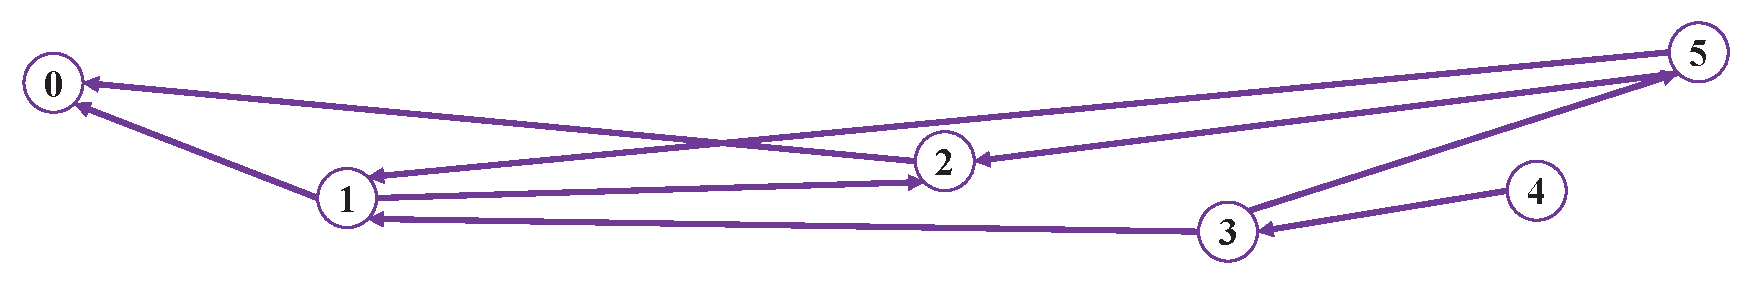
\includegraphics[scale=0.3]{pic/graph2.eps}
	\end{figure}
	\begin{equation}
		\setlength{\arraycolsep}{2pt}
		\begin{aligned}
			\vec{\textbf{h}}^{\left(1\right)}_1&=\sigma\left(\text{MEAN}\left(\vec{\textbf{h}}^{\left(0\right)}_1,\vec{\textbf{h}}^{\left(0\right)}_3,\vec{\textbf{h}}^{\left(0\right)}_5\right)\cdot\textbf{W}^{\left(0\right)}\right) \\
			&=\sigma\left(\begin{bmatrix}
				\frac{-0.5+1.7+0.8}{3} \\ \frac{1.3+2.2-0.9}{3}
			\end{bmatrix}^\top\begin{bmatrix}
				-0.0631 & 0.7147 \\
				-0.2050 & -0.1241 \\
				1.4897 & 1.4090 \\
				1.4172 & 0.6715
			\end{bmatrix}^\top\right)=\begin{bmatrix}
			1.0062 \\
			0 \\
			3.0597 \\
			1.9297
			\end{bmatrix}^\top \\
			\vec{\textbf{h}}^{\left(1\right)}_1&=\vec{\textbf{h}}^{\left(1\right)}_1/\|\vec{\textbf{h}}^{\left(1\right)}_1\|_2=\begin{bmatrix}
				0.2680 & 0 & 0.8149 & 0.5139
			\end{bmatrix}
		\end{aligned}
	\end{equation}
\end{frame}

\begin{frame}{GraphSAGE链接预测——前向传播（续）}
	\begin{figure}
		\centering
		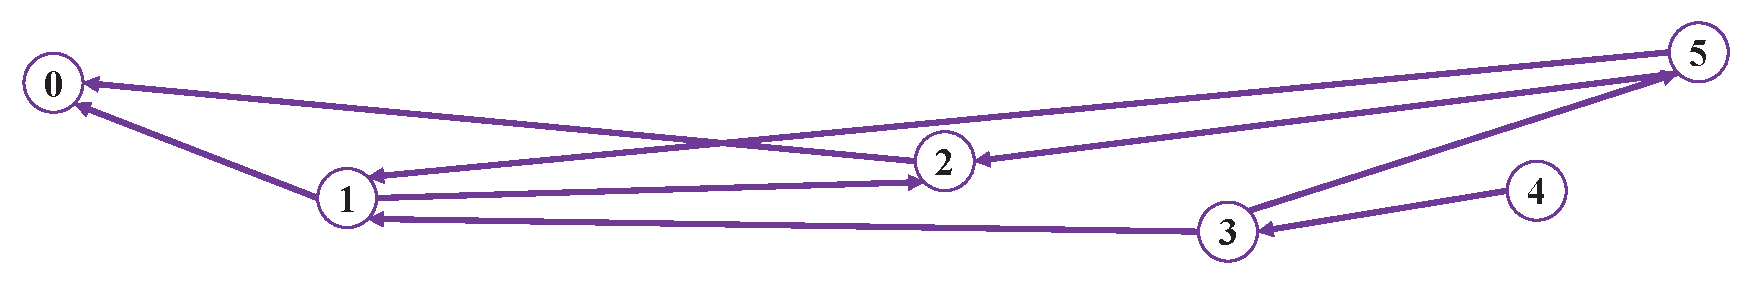
\includegraphics[scale=0.4]{pic/graph2.eps}
	\end{figure}
	\begin{equation}
		\setlength{\arraycolsep}{2pt}
		\textbf{H}^{\left(1\right)}=\begin{bmatrix}
			\vec{\textbf{h}}^{\left(1\right)}_0\\
			\vec{\textbf{h}}^{\left(1\right)}_1 \\
			\vec{\textbf{h}}^{\left(1\right)}_2 \\
			\vec{\textbf{h}}^{\left(1\right)}_3 \\
			\vec{\textbf{h}}^{\left(1\right)}_4 \\
			\vec{\textbf{h}}^{\left(1\right)}_5
		\end{bmatrix}
		=\begin{bmatrix}
			0.4163 & 0 & 0.8208 & 0.3912 \\
			0.2680 & 0 & 0.8149 & 0.5139 \\
			0.2342 & 0 & 0.8096 & 0.5383 \\
			0.1355 & 0 & 0.7866 & 0.6025 \\
			0 & 0 & 7122 & 0.7020 \\
			0.2044 & 0 & 0.8038 & 0.5587
		\end{bmatrix}       
	\end{equation}
\end{frame}

\begin{frame}{GraphSAGE链接预测——负采样}
	\begin{figure}
		\centering
		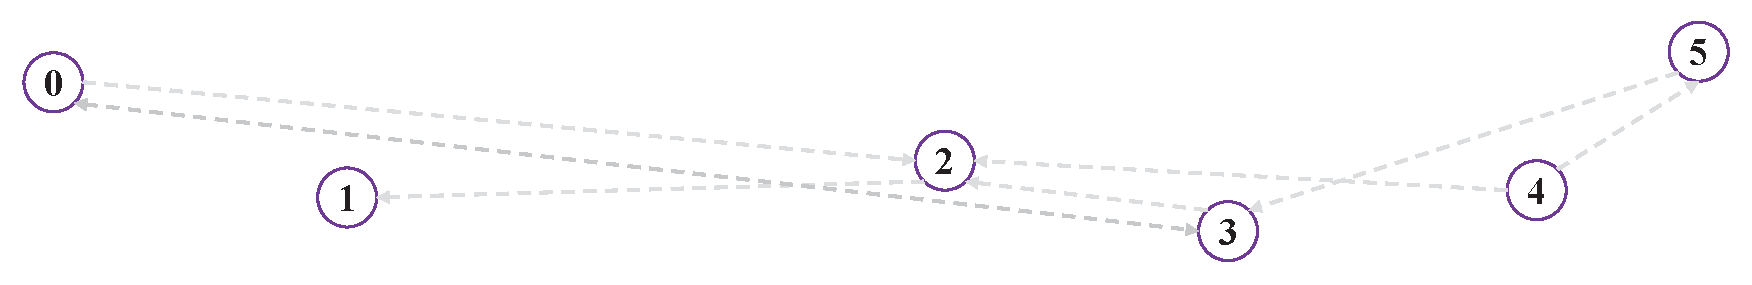
\includegraphics[scale=0.4]{pic/graph2n.eps}
	\end{figure}
	采样与原图中边数量相同的{\color{red}不存在边链接}（edge link）的节点对（pairs of nodes），形成非邻接矩阵（non-adjacency matrix）$\overline{\textbf{A}}$
	\begin{equation}
		\setlength{\arraycolsep}{2pt}
		\overline{\textbf{A}}=\begin{bmatrix}
			0 & 0 & 1 & 1 & 0 & 0 \\
			0 & 0 & 0 & 0 & 0 & 0 \\
			0 & 1 & 0 & 0 & 0 & 0 \\
			1 & 0 & 1 & 0 & 0 & 0 \\
			0 & 0 & 1 & 0 & 0 & 1 \\
			0 & 0 & 0 & 1 & 0 & 0
		\end{bmatrix}
	\end{equation}
\end{frame}

\begin{frame}{GraphSAGE链接预测——节点对点乘：原图}
	\begin{figure}
		\centering
		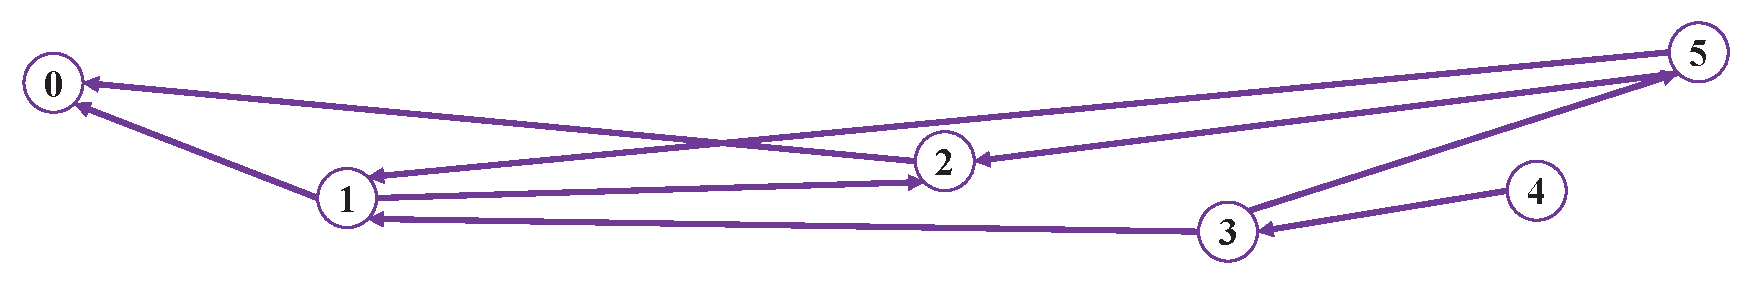
\includegraphics[scale=0.3]{pic/graph2.eps}
	\end{figure}
	对每一条边，计算源点的节点特征和汇点的节点特征的逐元素乘积（Hadamard product）后求和，得到边链接分数，以边$\left(5,2\right)$为例
	\begin{equation}
		\vec{\textbf{s}}_{\left(5,2\right)}=\text{SUM}\left(\begin{bmatrix}
			0.2044 \\
			0 \\
			0.8038 \\
			0.5587
		\end{bmatrix}^\top\otimes\begin{bmatrix}
		0.2342 \\
		0 \\
		0.8096 \\
		0.5383
		\end{bmatrix}^\top\right)=0.9993
	\end{equation}
\end{frame}

\begin{frame}{GraphSAGE链接预测——节点对点乘：负采样后的图}
	\begin{figure}
		\centering
		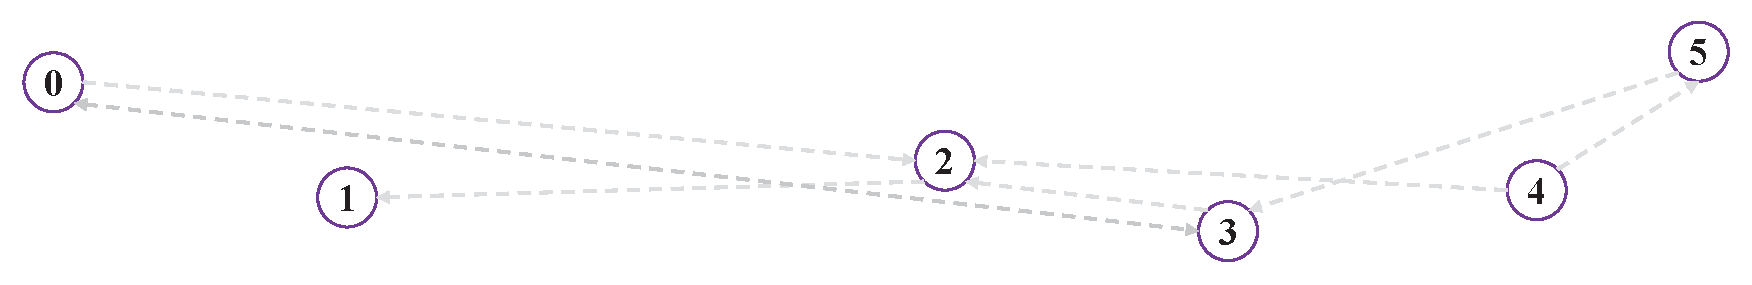
\includegraphics[scale=0.3]{pic/graph2n.eps}
	\end{figure}
	对每一条非边链接，计算源点的节点特征和汇点的节点特征的逐元素乘积（Hadamard product）后求和，得到非边链接分数
\end{frame}

\begin{frame}{GraphSAGE链接预测——计算损失}
	对原图和负采样后的图上计算的链接分数施加Sigmoid激活函数，得到链接概率
	\begin{equation}
		\setlength{\arraycolsep}{2pt}
		\vec{\textbf{p}}\left[0:7\right]=\text{Sigmoid}\left(\vec{\textbf{s}}\left[0:7\right]\right)=\text{Sigmoid}\left(\begin{bmatrix}
			\vec{\textbf{s}}_{\left(1,0\right)} \\
			\vec{\textbf{s}}_{\left(2,3\right)} \\
			\vec{\textbf{s}}_{\left(3,1\right)} \\
			\vec{\textbf{s}}_{\left(4,2\right)} \\
			\vec{\textbf{s}}_{\left(4,6\right)} \\
			\vec{\textbf{s}}_{\left(5,4\right)} \\
			\vec{\textbf{s}}_{\left(6,2\right)} \\
			\vec{\textbf{s}}_{\left(6,3\right)}             
		\end{bmatrix}\right)=\begin{bmatrix}             
			0.7274 \\
			0.7309 \\
			0.7256 \\
			0.7285 \\
			0.7304 \\
			0.7277 \\
			0.7305 \\
			0.7309
		\end{bmatrix}
	\end{equation}
\end{frame}

\begin{frame}{GraphSAGE链接预测——计算损失（续）}
	\begin{equation}
		\setlength{\arraycolsep}{2pt}
		\vec{\textbf{p}}\left[8:15\right]=\text{Sigmoid}\left(\vec{\textbf{s}}\left[8:15\right]\right)=\text{Sigmoid}\left(\begin{bmatrix}
			\vec{\textbf{s}}_{\left(0,2\right)} \\
			\vec{\textbf{s}}_{\left(0,3\right)} \\
			\vec{\textbf{s}}_{\left(2,1\right)} \\
			\vec{\textbf{s}}_{\left(3,0\right)} \\
			\vec{\textbf{s}}_{\left(3,2\right)} \\
			\vec{\textbf{s}}_{\left(4,2\right)} \\
			\vec{\textbf{s}}_{\left(4,5\right)} \\
			\vec{\textbf{s}}_{\left(5,3\right)}             
		\end{bmatrix}\right)=\begin{bmatrix}             
			0.7256 \\
			0.7186 \\
			0.7309 \\
			0.7186 \\
			0.7296 \\
			0.7220 \\
			0.7241 \\
			0.7304 
		\end{bmatrix}
	\end{equation}
	链接预测问题转换为边链接、非边链接二分类问题，损失使用交叉熵函数计算
	\begin{equation}
		\begin{aligned}
			\mathcal{L}&=-\frac{1}{16}\sum\limits_{i=0}^{7}\log\left(\vec{\textbf{s}}\left[i\right]\right)-\sum\limits_{j=8}^{15}\log\left(\vec{\textbf{s}}\left[j\right]\right)\\
			&\approx2.0754
		\end{aligned}
	\end{equation}
\end{frame}

\section{图注意力网络（GAT）}

\begin{frame}{回顾：Transformer中的自注意力机制~\cite{3b1ba2024}}
	\begin{figure}
		\centering
		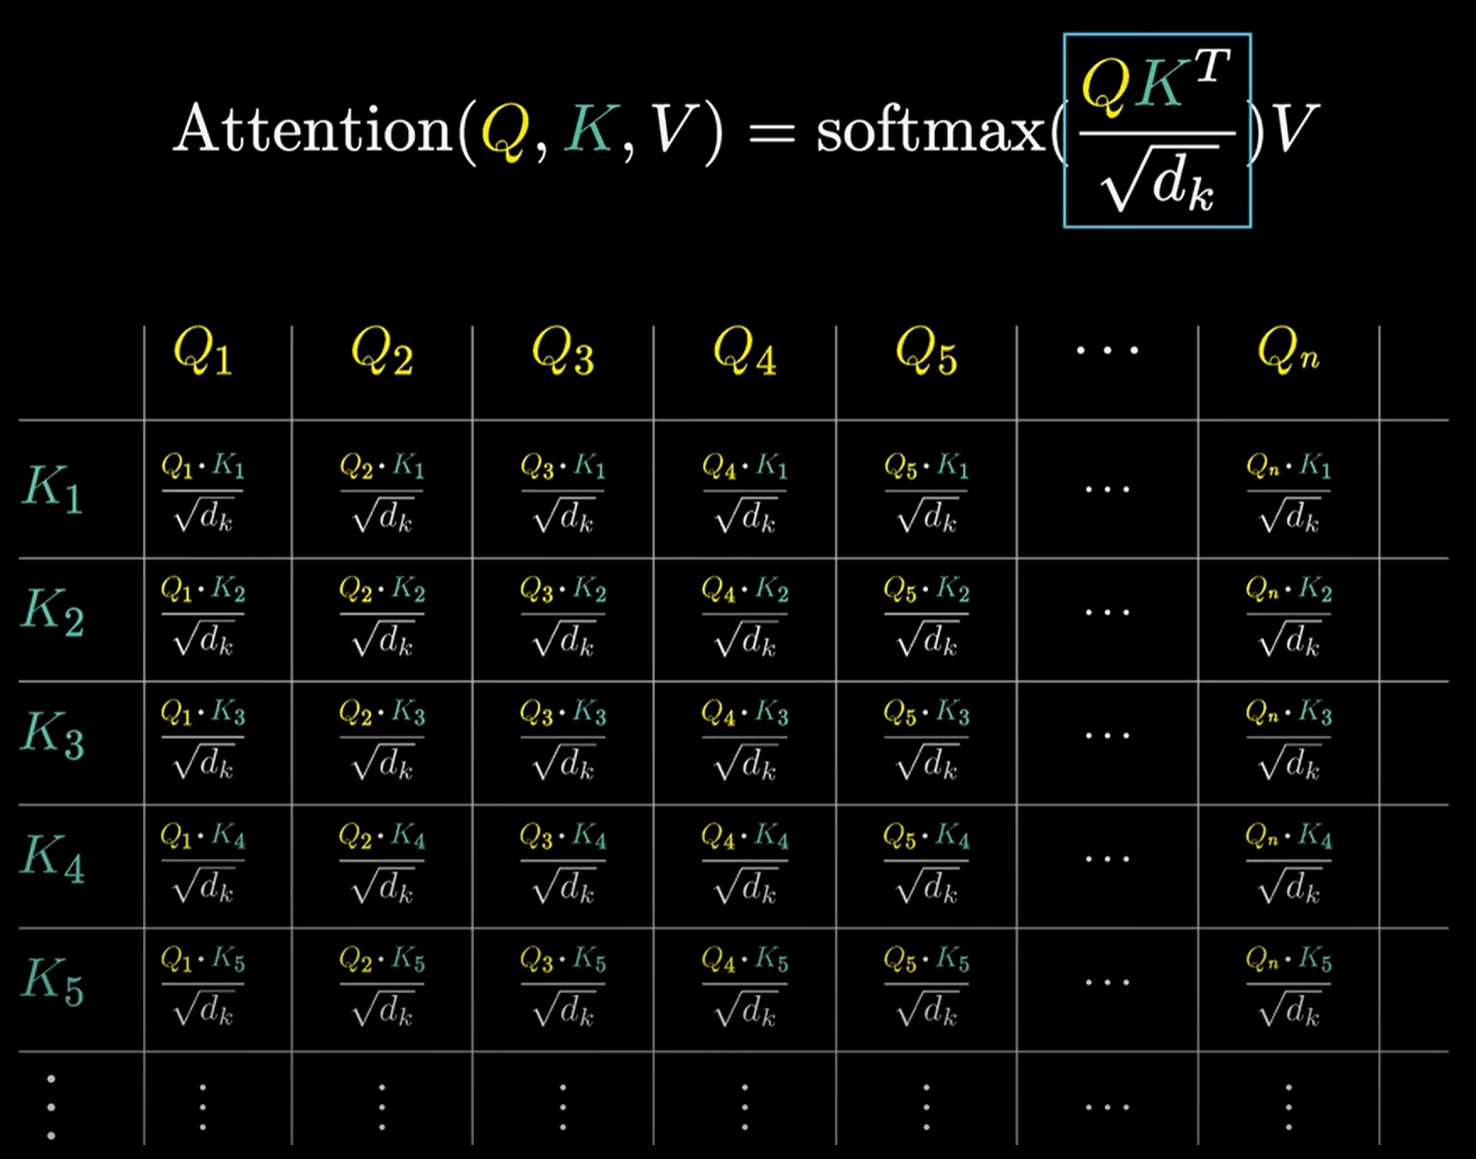
\includegraphics[scale=0.3]{pic/selfattr1.png}
	\end{figure}
\end{frame}

\begin{frame}{回顾：Transformer中的自注意力机制（续）}
	\begin{figure}
		\centering
		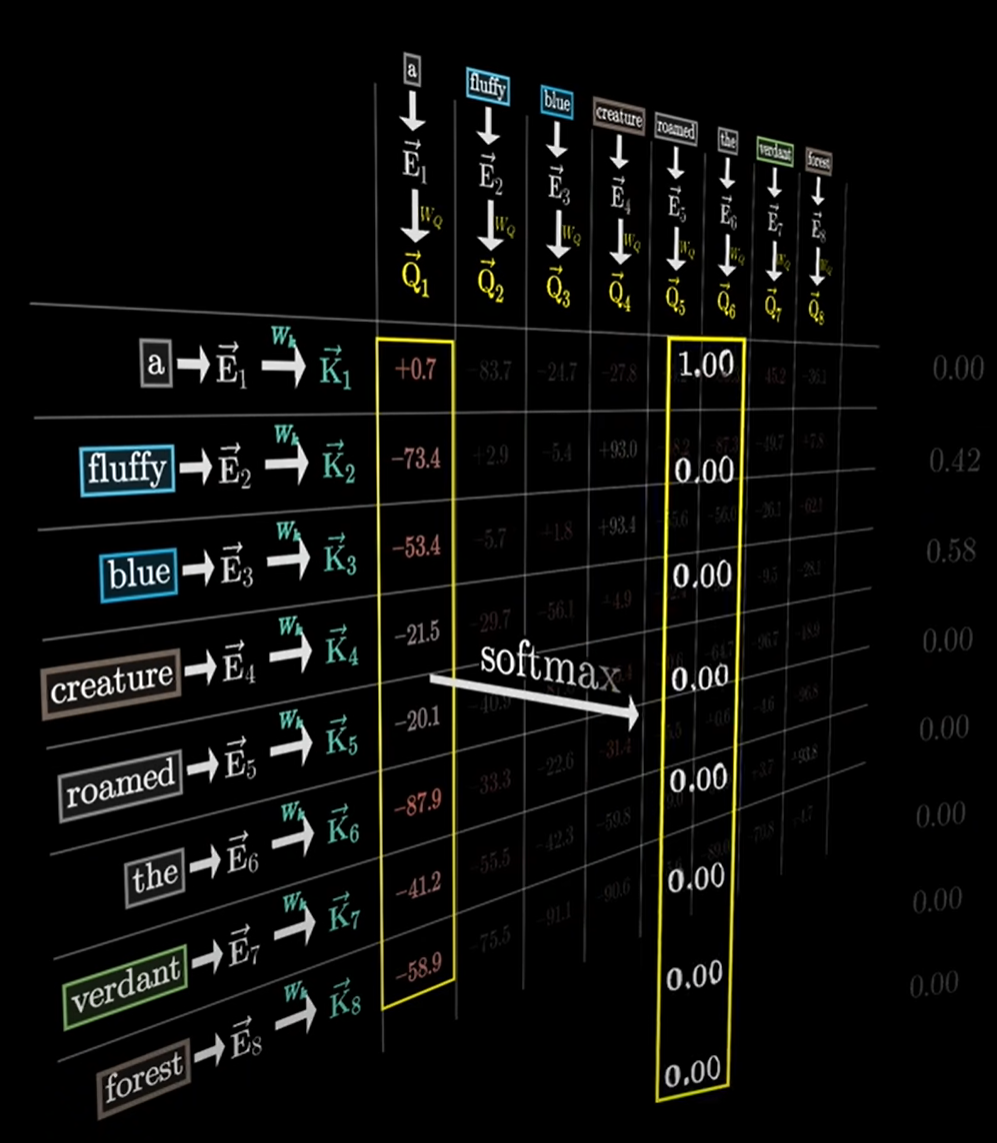
\includegraphics[scale=0.3]{pic/selfattr2.png}
	\end{figure}
\end{frame}

\begin{frame}{回顾：Transformer中的自注意力机制（续）}
	\begin{figure}
		\centering
		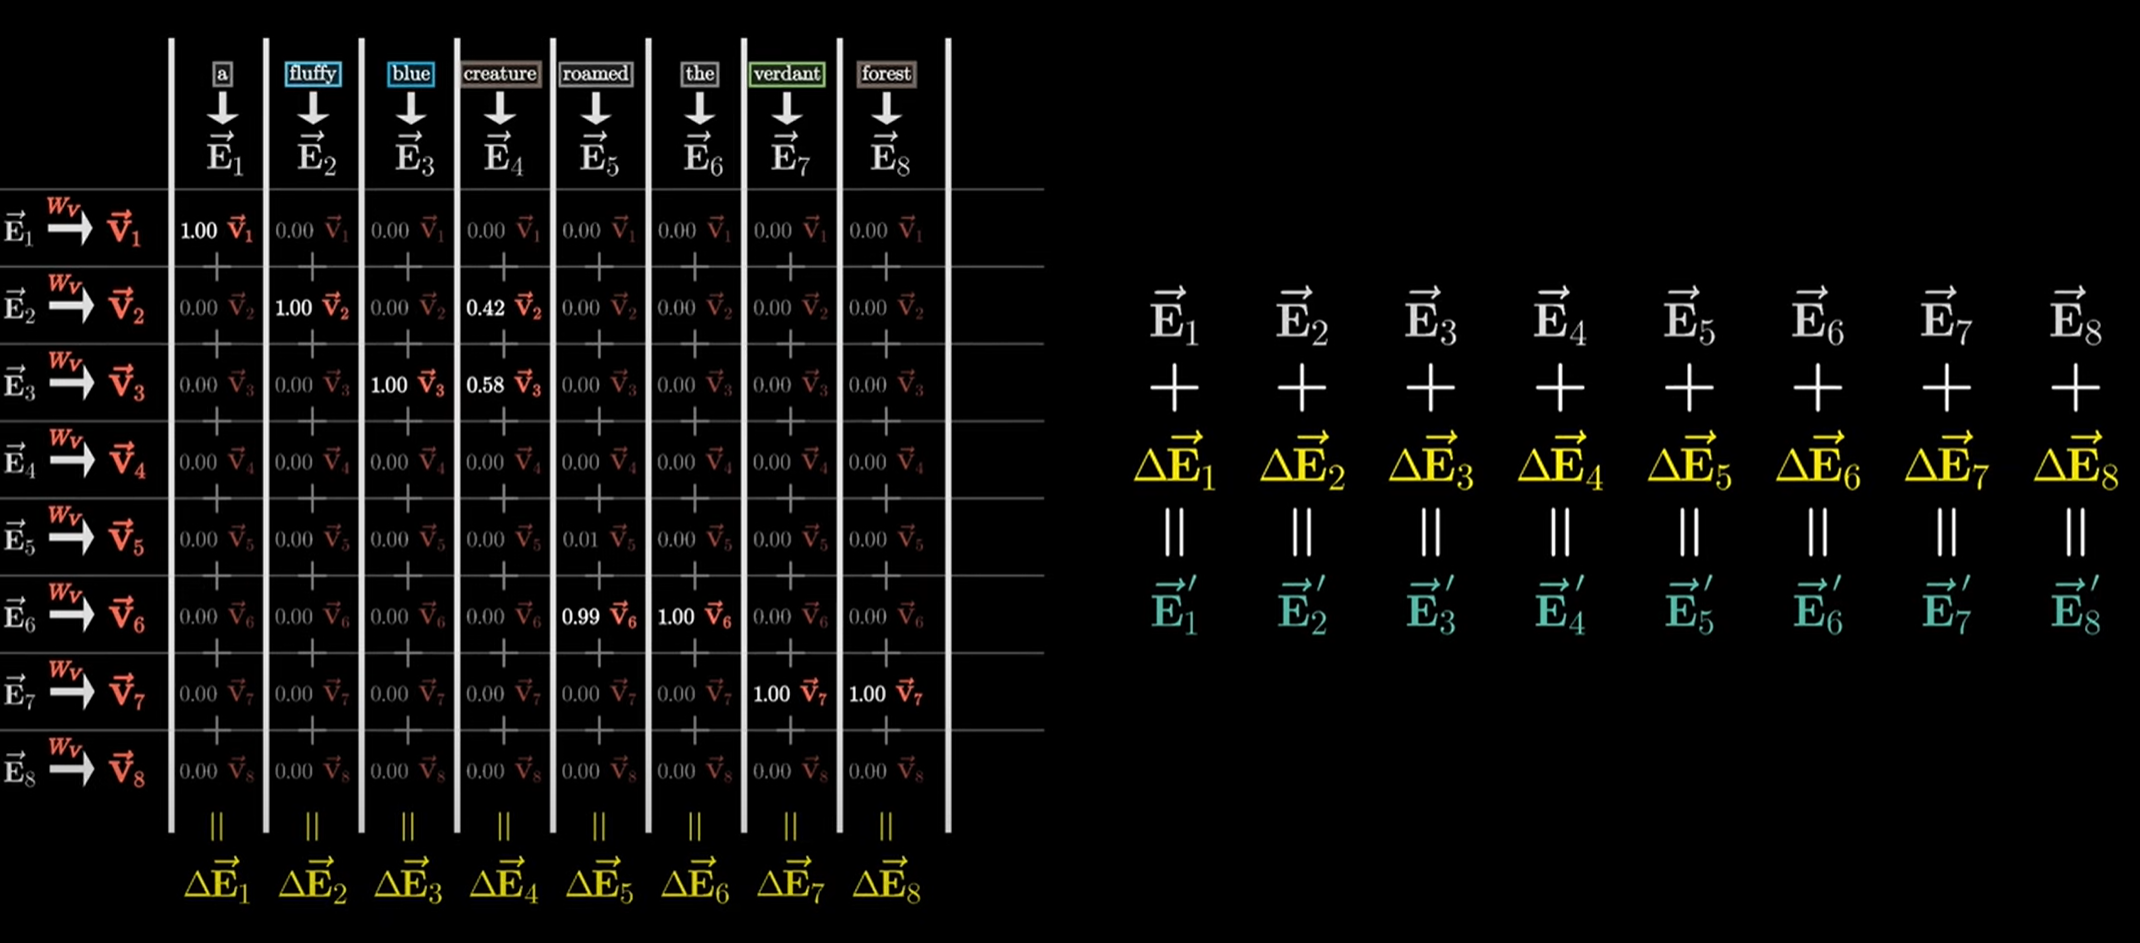
\includegraphics[scale=0.35]{pic/selfattr3.png}
	\end{figure}
\end{frame}

\begin{frame}{GAT中的自注意力机制}
	在图$\mathscr{G}$上的任意节点上执行自注意力（perform self-attention），计算得到{\color{red}注意力系数（attention coefficients）}
	\begin{equation}
		\label{eq:selfattr}
		\vec{\textbf{e}}_{ij}=\text{LeakyReLU}\left(\text{att\_node}^{\left(\ell\right)}\left(\left[\vec{\textbf{h}}^{\left(\ell\right)}_i\textbf{W}^{\left(\ell\right)}\|\vec{\textbf{h}}^{\left(\ell\right)}_j\textbf{W}^{\left(\ell\right)}\right]\right)\right),
	\end{equation}
	其中，$\text{att\_node}^{\left(\ell\right)}\left(\cdot\right)$是第$\ell$个隐含层的单层前馈神经网络（single-layer feedforward neural network）。\\
	{\color{red}\textbf{注意力系数刻画了节点$j$的特征对节点$i$的重要性}}。
\end{frame}

\begin{frame}{回顾：Transformer中的掩码注意力机制~\cite{3b1ba2024}}
	\begin{figure}
		\centering
		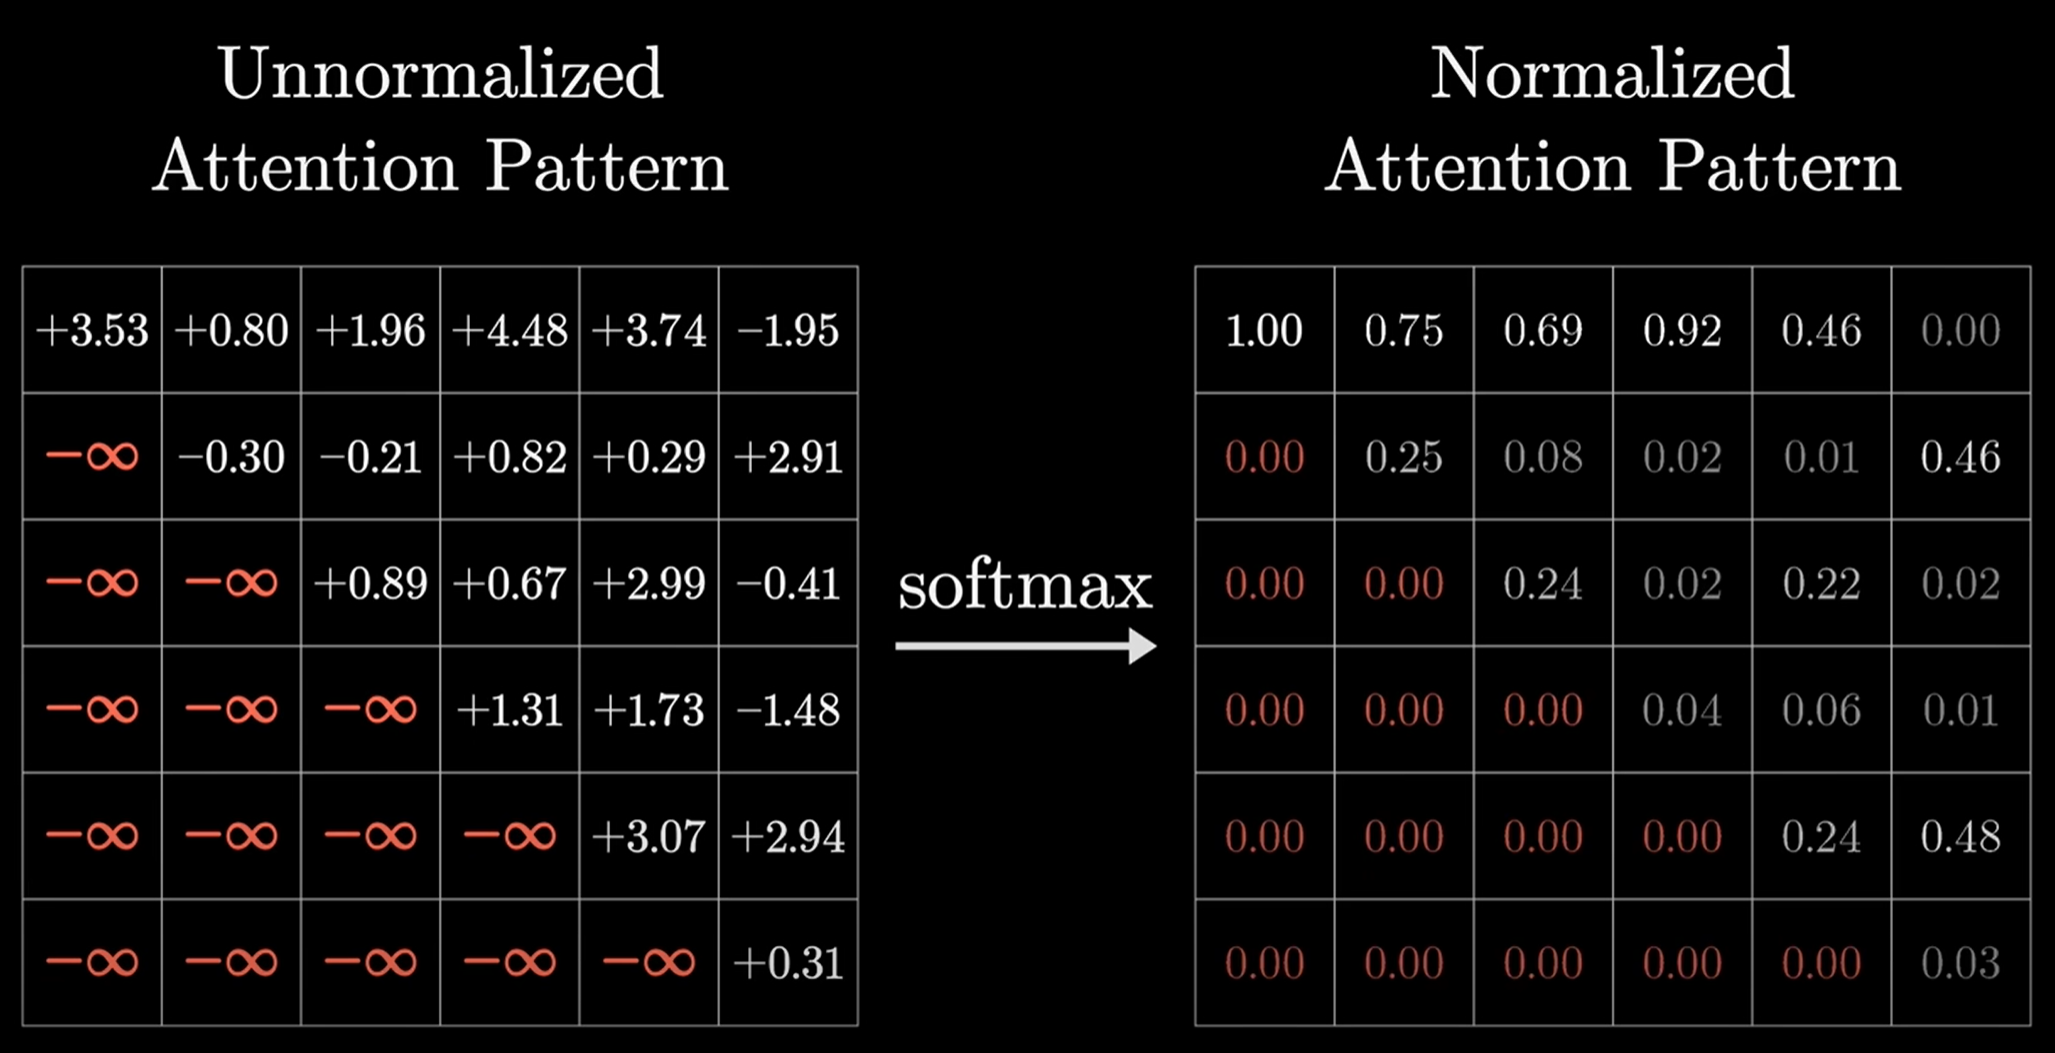
\includegraphics[scale=0.33]{pic/mask.png}
	\end{figure}
\end{frame}

\begin{frame}{GAT中的掩码注意力机制}
	在公式\ref{eq:selfattr}中，图的拓扑结构没有考虑进去，即任意两个节点间都能计算得到注意力系数。GAT中的{\color{red}掩码注意力机制}为仅计算邻接的节点之间的注意力系数，并使用Softmax进行归一化
	\begin{equation}
		\vec\alpha_{ij}=\text{Softmax}\left(\vec{\textbf{e}}_{ij}\right)=\frac{\exp\left(\vec{\textbf{e}}_{ij}\right)}{\sum\limits_{k\in\mathcal{N}\left(i\right)}\exp\left(\vec{\textbf{e}}_{ik}\right)}
	\end{equation}
\end{frame}

\begin{frame}{GAT中的消息传递}
	所有的$\vec\alpha_{ij}$得到后，计算第$\ell$层的输出（第$\ell+1$层的输入）
	\begin{equation}
		\vec{\textbf{h}}^{\left(\ell+1\right)}_i=\sigma\left(\sum\limits_{j\in\mathcal{N}\left(i\right)}\vec\alpha_{ij}\vec{\textbf{h}}^{\left(\ell\right)}_i\textbf{W}^{\left(\ell\right)}\right).
	\end{equation}
	回顾GCN的消息传递形式
	\begin{equation*}
		\vec{\textbf{h}}_i^{\left(\ell+1\right)}=\sigma\left(\sum\limits_{j\in\mathcal{N}\left(i\right)}\frac{1}{c_{ij}}\vec{\textbf{h}}_j^{\left(\ell\right)}\textbf{W}^{\left(\ell\right)}\right),
	\end{equation*}
	可以看出，GAT在对邻居节点特征聚合时引入了注意力机制。
\end{frame}

\begin{frame}{回顾：Transformer中的多头注意力机制~\cite{3b1ba2024}}
	\begin{figure}
		\centering
		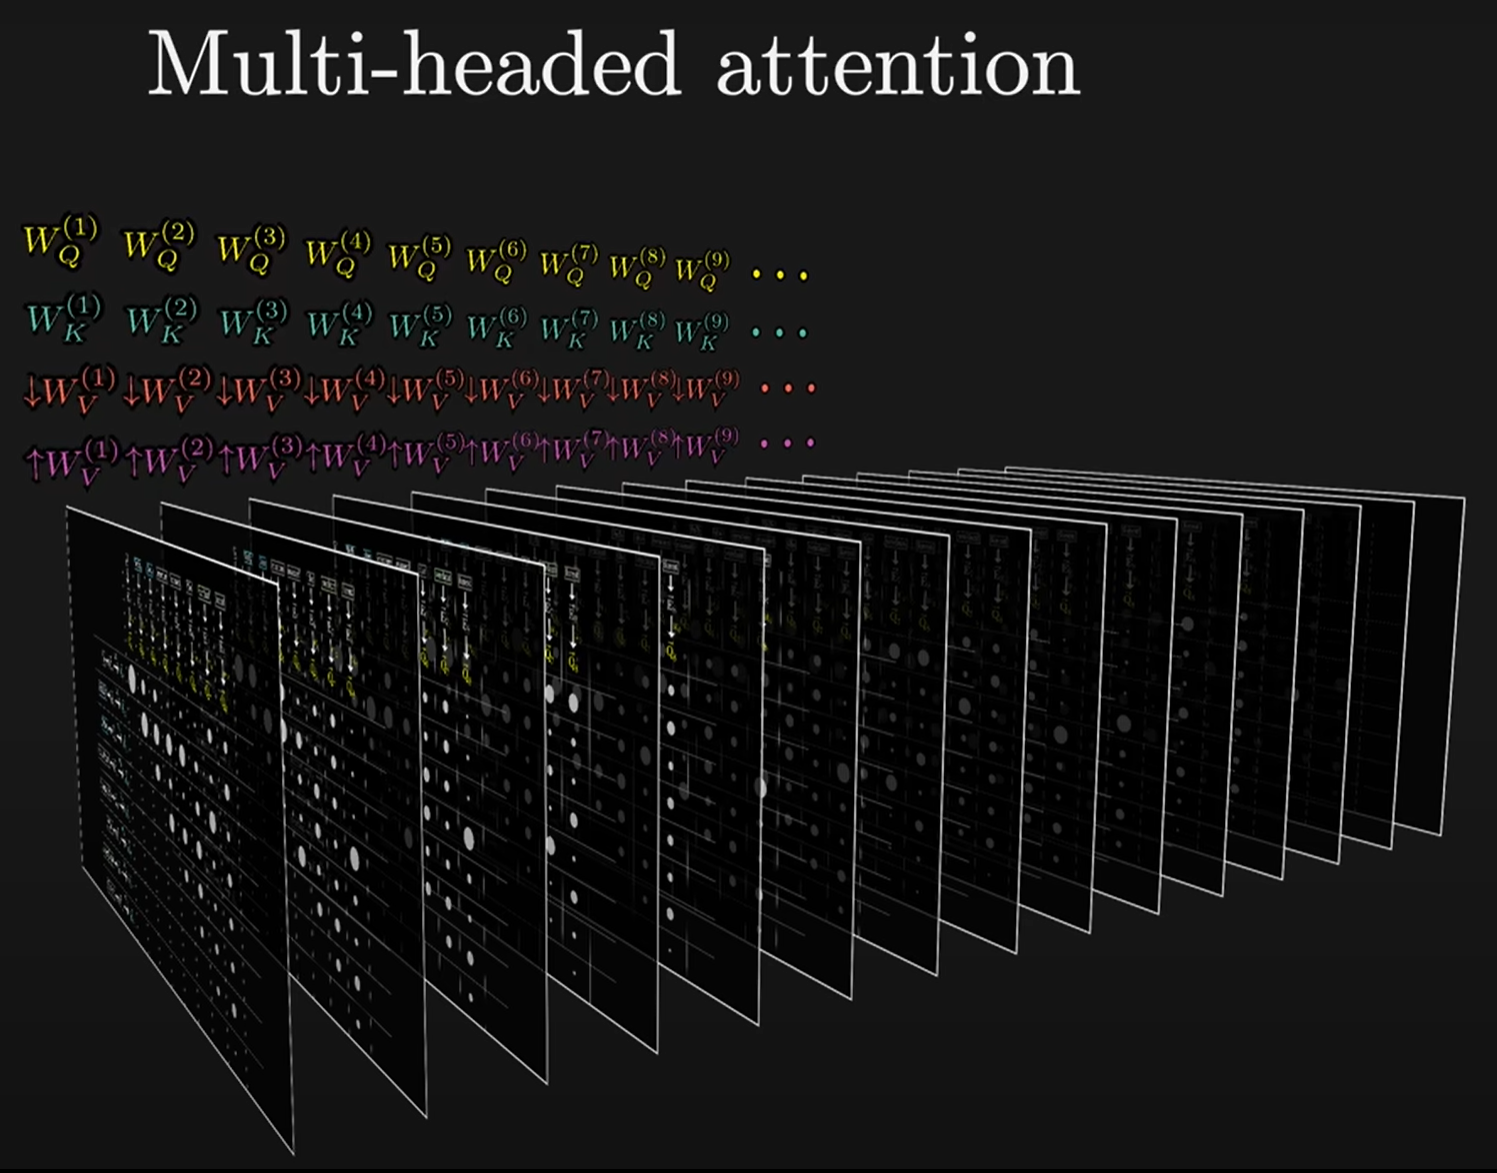
\includegraphics[scale=0.3]{pic/multihead.png}
	\end{figure}
\end{frame}

\begin{frame}{GAT中的多头注意力机制}
	K个不同的注意力机制并行执行
	\begin{equation}
		\vec{\textbf{h}}^{\left(\ell+1\right)}_i=\mathop{\|}\limits_{k=1}^K\sigma\left(\sum\limits_{j\in\mathcal{N}\left(i\right)}\vec\alpha_{ij}^k\vec{\textbf{h}}^{\left(\ell\right)}_i\textbf{W}^{\left(\ell\right)^k}\right).
	\end{equation}
\end{frame}

\begin{frame}{将边特征融入注意力机制}
	在DGL和PyG框架实现的GAT中，边的特征也可以添加到注意力系数的计算中
	\begin{equation}
		\vec{\textbf{e}}_{ij}=\text{LeakyReLU}\left(\text{att\_node}^{\left(\ell\right)}\left(\left[\vec{\textbf{h}}^{\left(\ell\right)}_i\textbf{W}^{\left(\ell\right)}\|\vec{\textbf{h}}^{\left(\ell\right)}_j\textbf{W}^{\left(\ell\right)}\right]\right)+\text{att\_edge}^{\left(\ell\right)}\left(\vec{\textbf{g}}_{ij}\textbf{W}'^{\left(\ell\right)}\right)\right),
	\end{equation}
	其中，$\vec{\textbf{g}}_{ij}$为边$\left(i,j\right)$的特征行向量，$\textbf{W}'^{\left(\ell\right)}$为第$\ell$层应用于边特征上的权重矩阵，$\text{att\_edge}^{\left(\ell\right)}\left(\cdot\right)$是第$\ell$个隐含层的{\color{red}另一个}单层前馈神经网络。
\end{frame}

\section{图同构网络（GIN）}

\begin{frame}{输入图：批处理图}
	为减少I/O操作，加快图神经网络训练和推理，以图为中心的任务（graph-focused task）通常将若干张小图“打包”成批处理图（batched graph）。如下图所示，图$\mathscr{G}_1$和图$\mathscr{G}_2$
	\begin{figure}
		\centering
		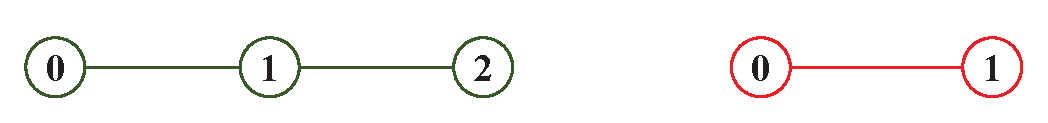
\includegraphics[scale=0.5]{pic/batch.eps}
	\end{figure}
	其组成的批处理图的邻接矩阵$\textbf{A}$、初始节点特征矩阵$\textbf{H}^{\left(0\right)}$和批处理向量$\vec{\textbf{q}}$为：
	\begin{equation}
		\setlength{\arraycolsep}{2pt}
		\begin{matrix}
			\begin{matrix}
				\textbf{A}=\begin{pmatrix}
					{\color{deepgreen}0} & {\color{deepgreen}1} & {\color{deepgreen}0} & 0 & 0 \\
					{\color{deepgreen}1} & {\color{deepgreen}0} & {\color{deepgreen}1} & 0 & 0 \\
					{\color{deepgreen}0} & {\color{deepgreen}1} & {\color{deepgreen}0} & 0 & 0 \\
					0 & 0 & 0 & {\color{red}0} & {\color{red}1} \\
					0 & 0 & 0 & {\color{red}1} & {\color{red}0} 
				\end{pmatrix} &
				\textbf{H}^{\left(0\right)}=\begin{pmatrix}
					{\color{deepgreen}-1.0} & {\color{deepgreen}0.5}\\
					{\color{deepgreen}0.5} & {\color{deepgreen}0.7}\\
					{\color{deepgreen}1.3} & {\color{deepgreen}-0.1}\\
					{\color{red}0} & {\color{red}1.2} \\
					{\color{red}2.3} & {\color{red}0.9} 
				\end{pmatrix}
			\end{matrix}\\
			\vec{\textbf{q}}=\begin{pmatrix}
				{\color{deepgreen}0} & {\color{deepgreen}0} & {\color{deepgreen}0} & {\color{red}1} & {\color{red}1}
			\end{pmatrix}
		\end{matrix}
	\end{equation}
\end{frame}

\begin{frame}{卷积层}
	与标准GCN的逐层传播规则类似，图同构网络（graph isomorphism network，GIN）的逐层传播规则定位为：
	\begin{equation}
		\textbf{H}^{\left(\ell+1\right)}=\text{MLP}^{\left(\ell\right)}\left(\textbf{A}\textbf{H}^{\left(\ell\right)}\right),
	\end{equation}
	$\text{MLP}\left(cdot\right)$为多层感知机，其输入为$\textbf{A}\textbf{H}^{\left(\ell\right)}$。
	
	此处使用MLP的原因~\cite{xu2019gin}将在下一部分详细展开讨论。
\end{frame}

\begin{frame}{图池化层（图读出层）}
	图分类任务的基本思想为{\color{red}\textbf{将图分类问题转换为节点分类问题}}，得到最终的节点嵌入表示后，需要对图的嵌入表示（特征）进行提取。
	
	类似于神经网络中的池化（pooling）操作，图特征$\vec{\textbf{F}}$的提取过程采用图池化（graph pooling）（图读出（graph-level readout），如下图进行最大（max）图池化操作
	\begin{equation}
		\setlength{\arraycolsep}{2pt}
		\begin{matrix}
			\begin{matrix}
				\textbf{H}^{\left(0\right)}=\begin{pmatrix}
					{\color{deepgreen}0.255} & {\color{deepgreen}1.721}\\
					{\color{deepgreen}0} & {\color{deepgreen}1.022}\\
					{\color{deepgreen}1.311} & {\color{deepgreen}0.981}\\
					{\color{red}4.232} & {\color{red}0.756} \\
					{\color{red}1.577} & {\color{red}0} 
				\end{pmatrix} \\
				\vec{\textbf{q}}=\begin{pmatrix}
					{\color{deepgreen}0} & {\color{deepgreen}0} & {\color{deepgreen}0} & {\color{red}1} & {\color{red}1}
				\end{pmatrix}
			\end{matrix} &
			\textbf{F}=\begin{pmatrix}
				{\color{deepgreen}1.311} & {\color{deepgreen}1.721}\\
				{\color{red}4.232} & {\color{red}0.756}
			\end{pmatrix}
		\end{matrix}
	\end{equation}
\end{frame}

\begin{frame}{线性预测层~\cite{dmlc2023gin}}
	\begin{figure}
		\centering
		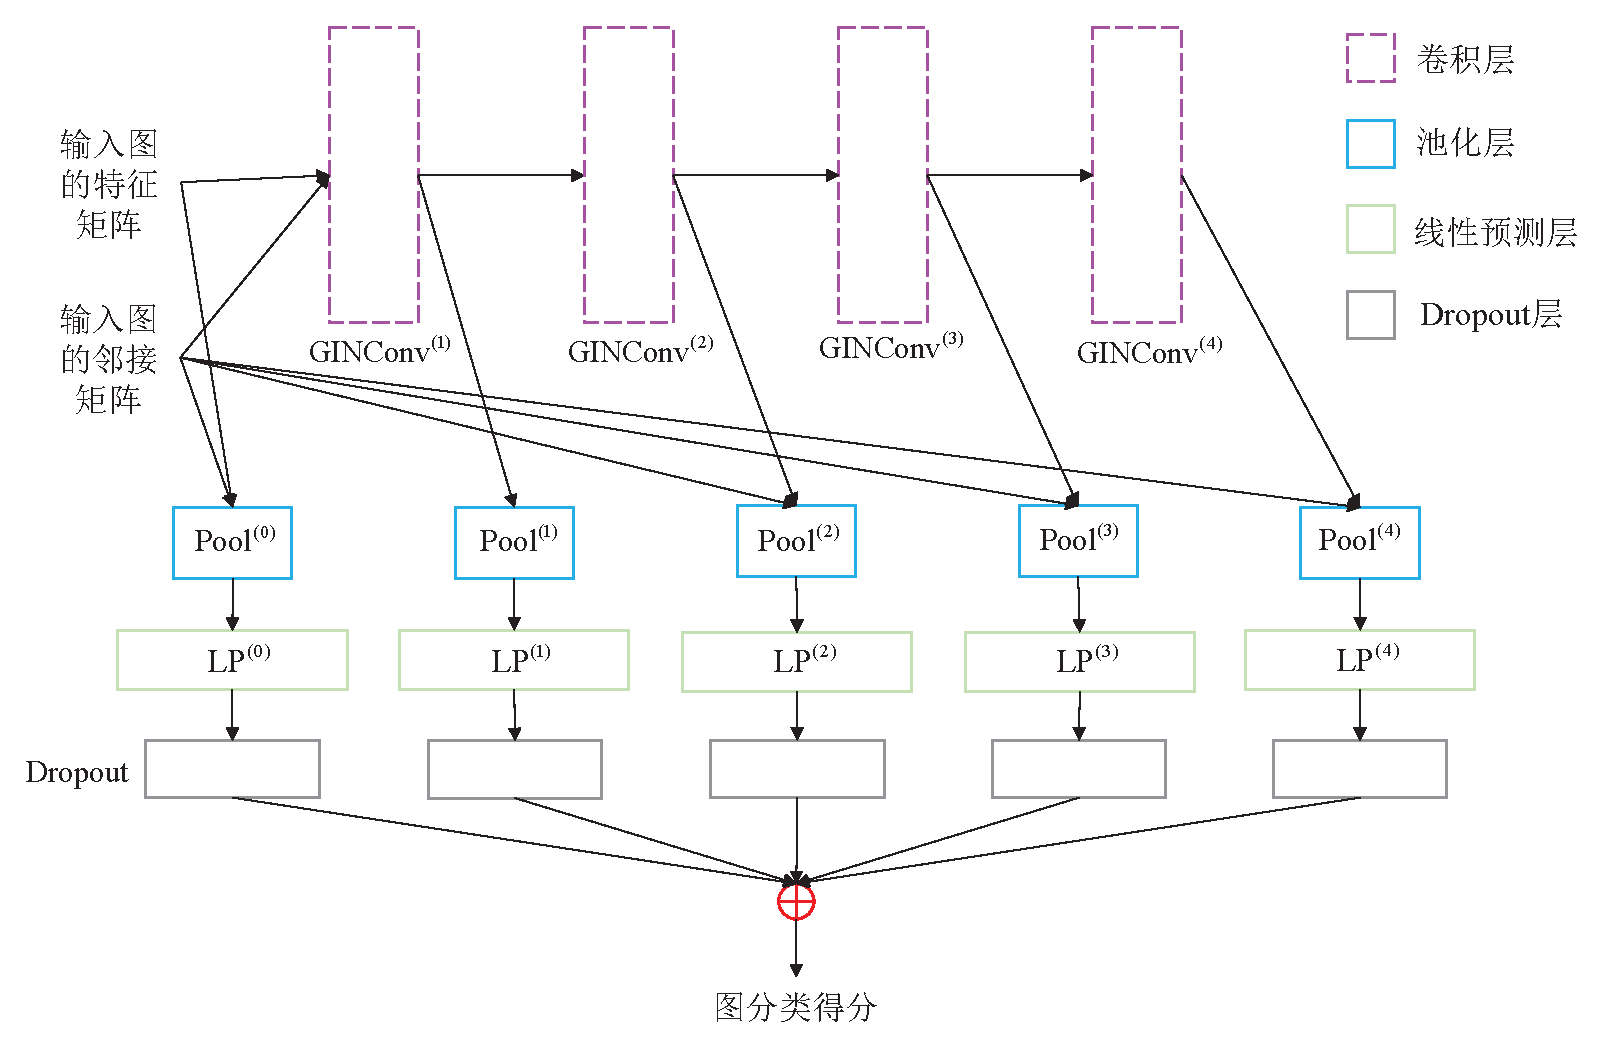
\includegraphics[scale=0.4]{pic/gin.eps}
	\end{figure}
\end{frame}


\section{图神经网络的能力：Weisfeiler-Lehman测试}


\begin{frame}{图同构问题}
	在图论中，如果图$\mathscr{G}_1\left(\mathscr{V}_1,\mathscr{E}_1\right)$和$\mathscr{G}_2\left(\mathscr{V}_2,\mathscr{E}_2\right)$之间存在边保留的双射（edge-preserving bijection）
	\begin{equation}
		f:\mathscr{V}_1\to \mathscr{V}_2,
	\end{equation}
	也即：图$\mathscr{G}_1$中的任意两个节点$u$和$v$是{\color{red}邻接的} {\color{red}\textbf{当且仅当}} $f\left(u\right)$和$f\left(v\right)$在图$\mathscr{G}_2$中是{\color{red}邻接的}，那么图$\mathscr{G}_1$和$\mathscr{G}_2$是同构的（isomorphic），记作$\mathscr{G}_1\cong\mathscr{G}_2$。
	\begin{figure}
		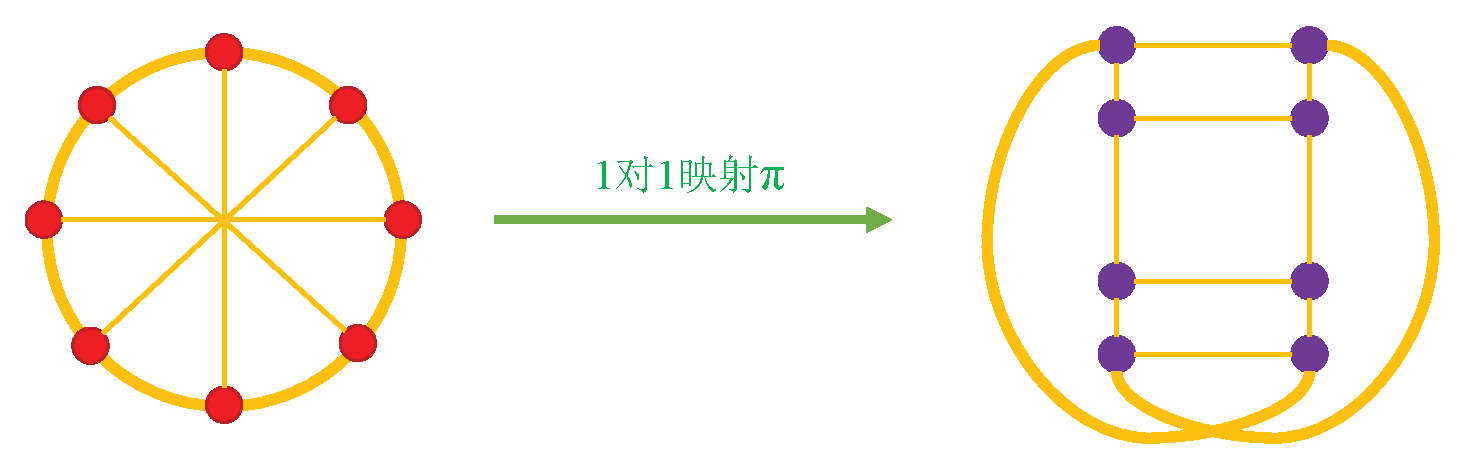
\includegraphics[scale=0.3]{pic/isog.eps}
	\end{figure}
	同构的图具有相同的连通性（connectivity），仅在节点的排序（permutation）上不同。
\end{frame}

\begin{frame}{节点颜色}
	\begin{formal}
		{\color{red}\textbf{节点颜色}}是一个函数$\mathscr{V}\to\Sigma$（$\Sigma$为任意到达域（codomain））。\\
		节点着色（node colored）或节点打标签（labeled）的图$\left(\mathscr{G}\right)$为具有节点着色$\mathscr{V}\to\Sigma$的图，$l\left(v\right)$为节点$v\in\mathscr{V}$的标签（label）或颜色（color）。\\
		{\color{red}\textbf{颜色细分}}：两种节点颜色$c_1$、$c_2$，如果$c_1\left(u\right)=c_1\left(v\right)\Longrightarrow c_2\left(u\right)=c_2\left(v\right)$，那么$c_1${\color{red}\textbf{细分（refines）}}$c_2$，记作$c_1\sqsubseteq c_2$。特别地，如果有$c_1\sqsubseteq c_2$且$c_2\sqsubseteq c_1$，则两种节点颜色等价（equivalent）。\\
		节点颜色$c$的{\color{red}\textbf{颜色类（color class）}}$Q\subseteq\mathscr{V}$是满足$c\left(u\right)=c\left(v\right)\,\forall u,v\in\mathscr{V}$的极大集（maximal set）。
	\end{formal}
\end{frame}

\begin{frame}{颜色细分}
	颜色细分（color refinement）~\cite{morgan1965description}（又称朴素顶点分类（naive vertex classification）、一维Weisfeiler-Lehman算法~\cite{weisfeiler1968reduction}）迭代计算图$\mathscr{G}$中所有节点的颜色。
	\begin{formal}
		\textbf{初始化}：所有节点初始化为同种颜色。\\
		\textbf{细分步骤}：对于任意两个节点$u$和$v$，如果存在一种颜色$c$，使得节点$u$和$v$有不同数量的颜色为$c$的邻居节点，那么节点$u$和$v$细分为不同的颜色。\\
		\textbf{终止条件}：当节点颜色（coloring）达到{\color{red}稳定状态}\footnote{连续两次迭代得到的节点划分（partition）相同}后，终止细分。
	\end{formal}
\end{frame}

\begin{frame}{1-WL}
	\begin{footnotesize}
		\begin{algorithm}[H]
			\label{algo:wl}
			\caption{\footnotesize 一维Weisfeiler-Lehman算法（1-WL）}
			\LinesNumbered
			\KwIn{初始节点颜色（标签） $c_l^{\left(0\right)}=l$}
			\KwOut{最终节点颜色（标签） $c_l^{\left(T\right)}$}
			$t\gets1$\;
			\While{True}{
				\For{$v\in\mathcal{V}$}{
					$c_l^{\left(t\right)}\gets\text{HASH}\left(c_l^{\left(t-1\right)}\left(v\right),\lbrace\!\!\lbrace c_l^{\left(t-1\right)}\left(u\right)|\,u\in\mathcal{N}_v\rbrace\!\!\rbrace\right)$\;
				}
				$t\gets t+1$\;
				\If{$c_l^{\left(t\right)}$和$c_l^{\left(t-1\right)}$所有像（images）组成的集合的势（cardinalities）相等}{
					$c_l^{\left(T\right)}=c_l^{\left(t\right)}$\;
					break\;
				}
			}
		\end{algorithm}
	\end{footnotesize}
\end{frame}

\begin{frame}{1-WL实例——第1次迭代}
	\begin{figure}
		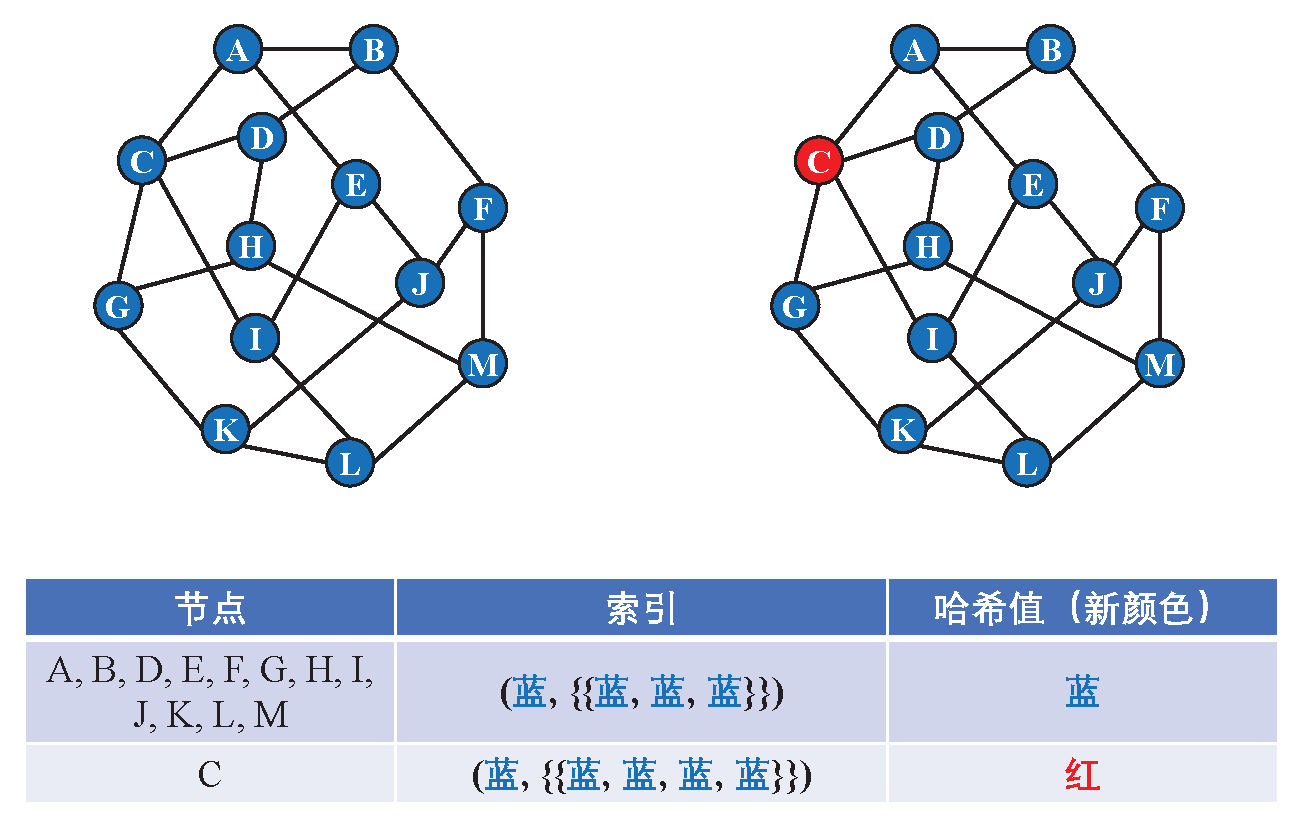
\includegraphics[scale=0.4]{pic/1wl-iter1.eps}
	\end{figure}
\end{frame}

\begin{frame}{1-WL实例——第2次迭代}
	\begin{figure}
		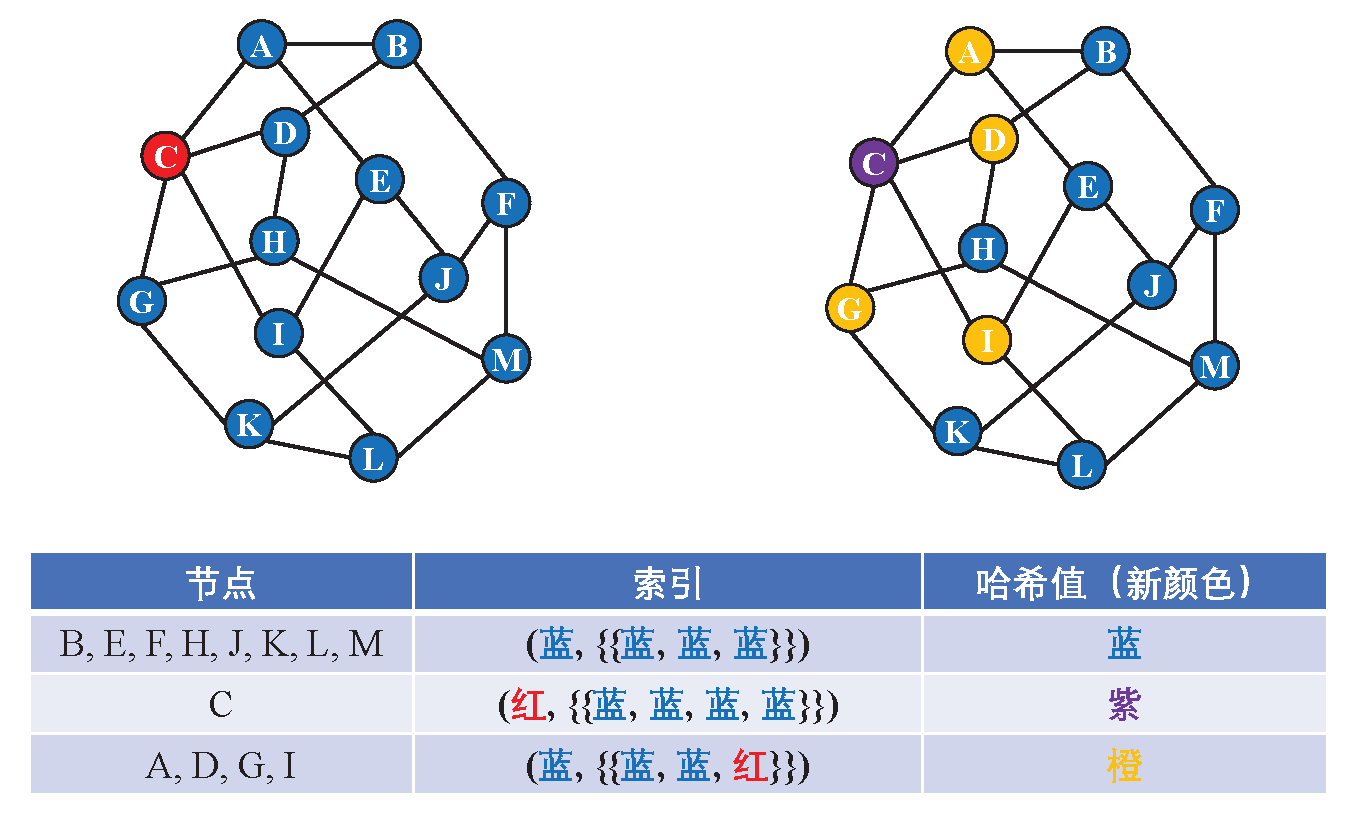
\includegraphics[scale=0.4]{pic/1wl-iter2.eps}
	\end{figure}
\end{frame}

\begin{frame}{1-WL实例——第3次迭代}
	\begin{figure}
		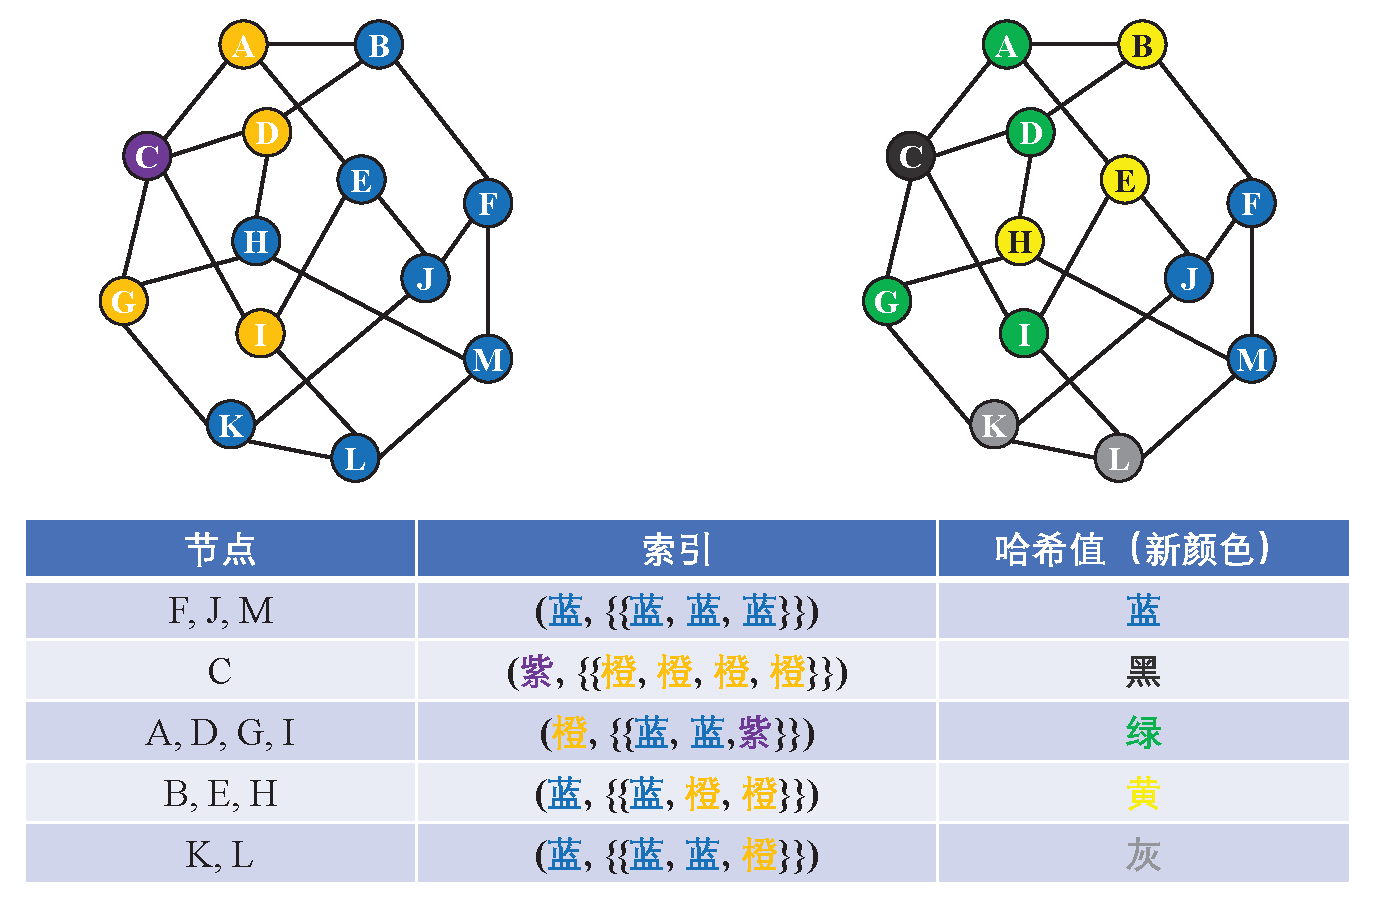
\includegraphics[scale=0.4]{pic/1wl-iter3.eps}
	\end{figure}
\end{frame}

\begin{frame}{1-WL实例——第4次迭代}
	\begin{figure}
		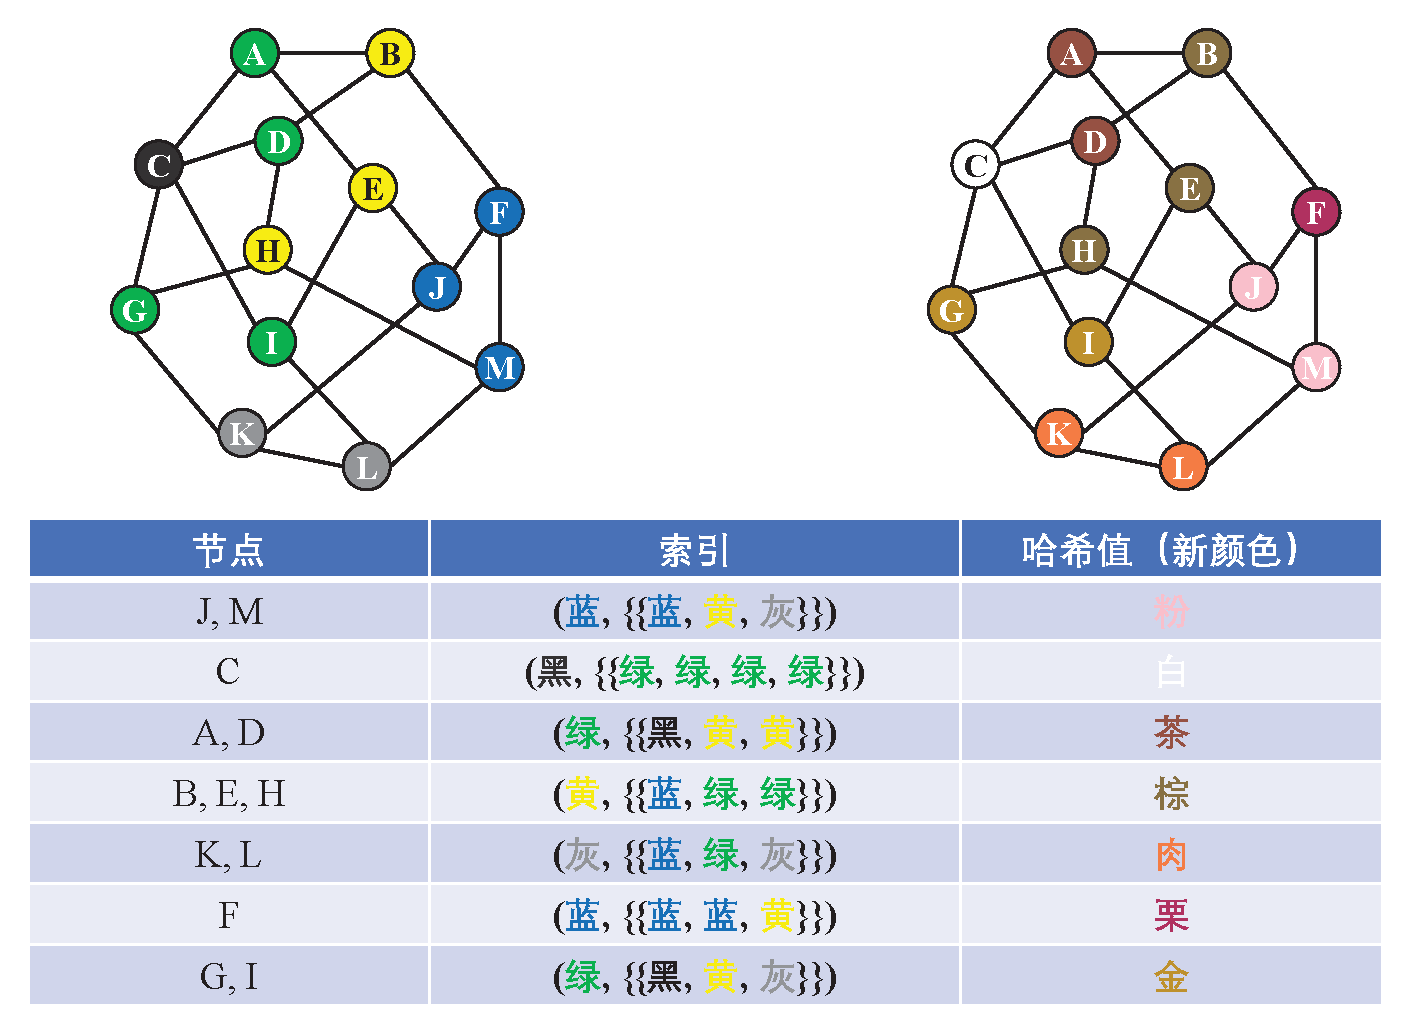
\includegraphics[scale=0.4]{pic/1wl-iter4.eps}
	\end{figure}
\end{frame}

\begin{frame}{1-WL实例——第5次迭代}
	\begin{figure}
		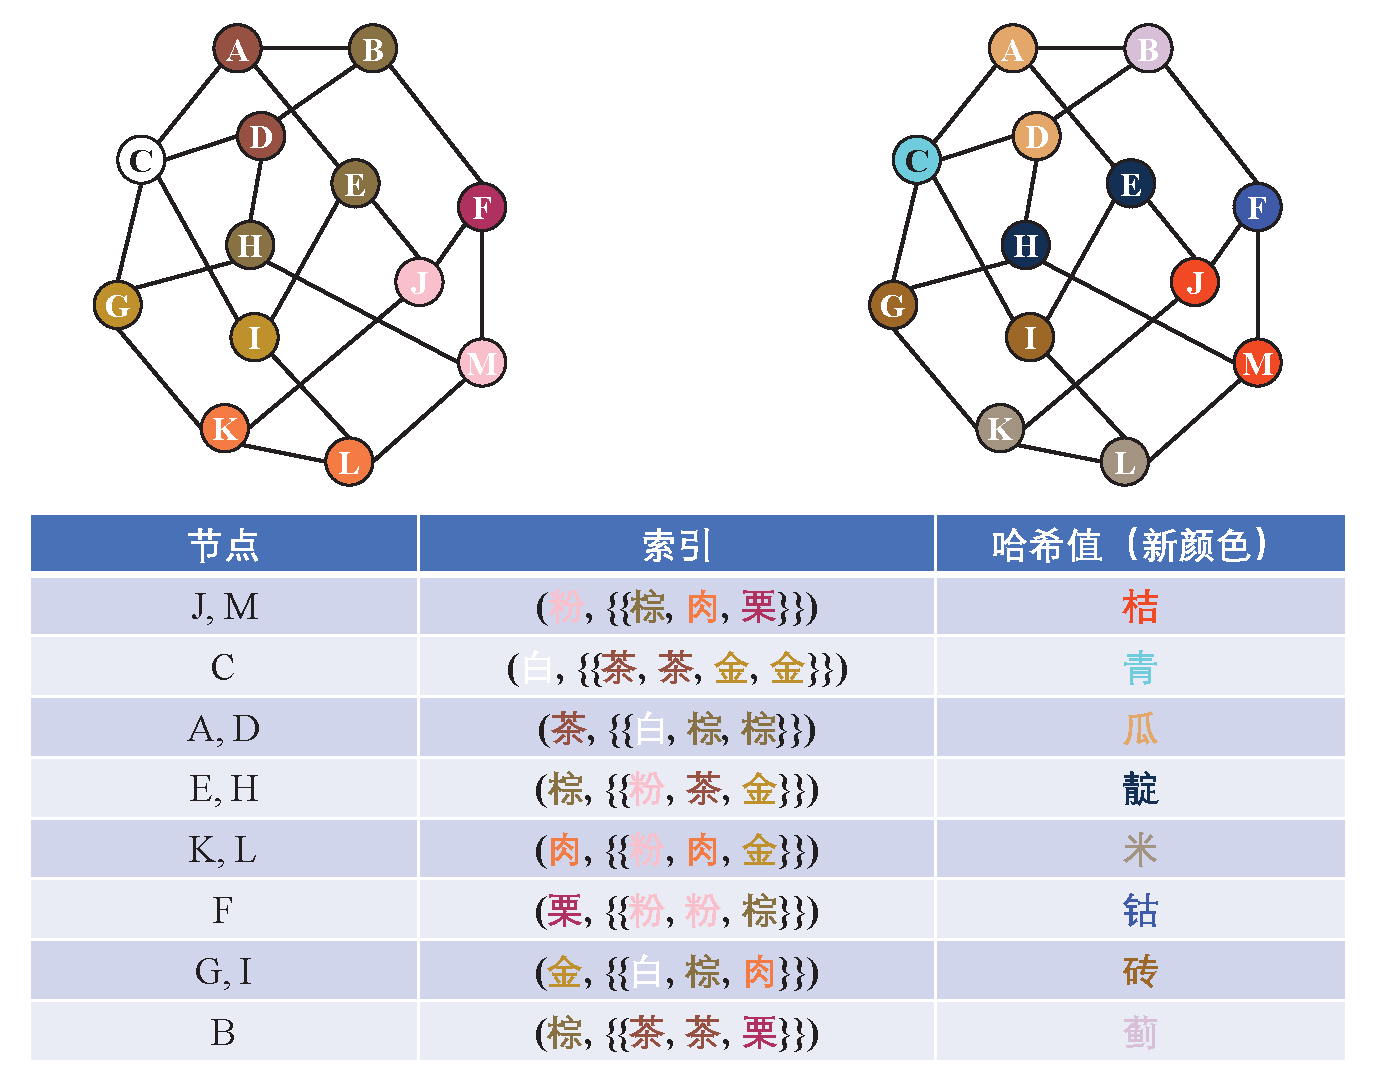
\includegraphics[scale=0.38]{pic/1wl-iter5.eps}
	\end{figure}
\end{frame}

\begin{frame}{1-WL实例——第6次迭代}
	\begin{figure}
		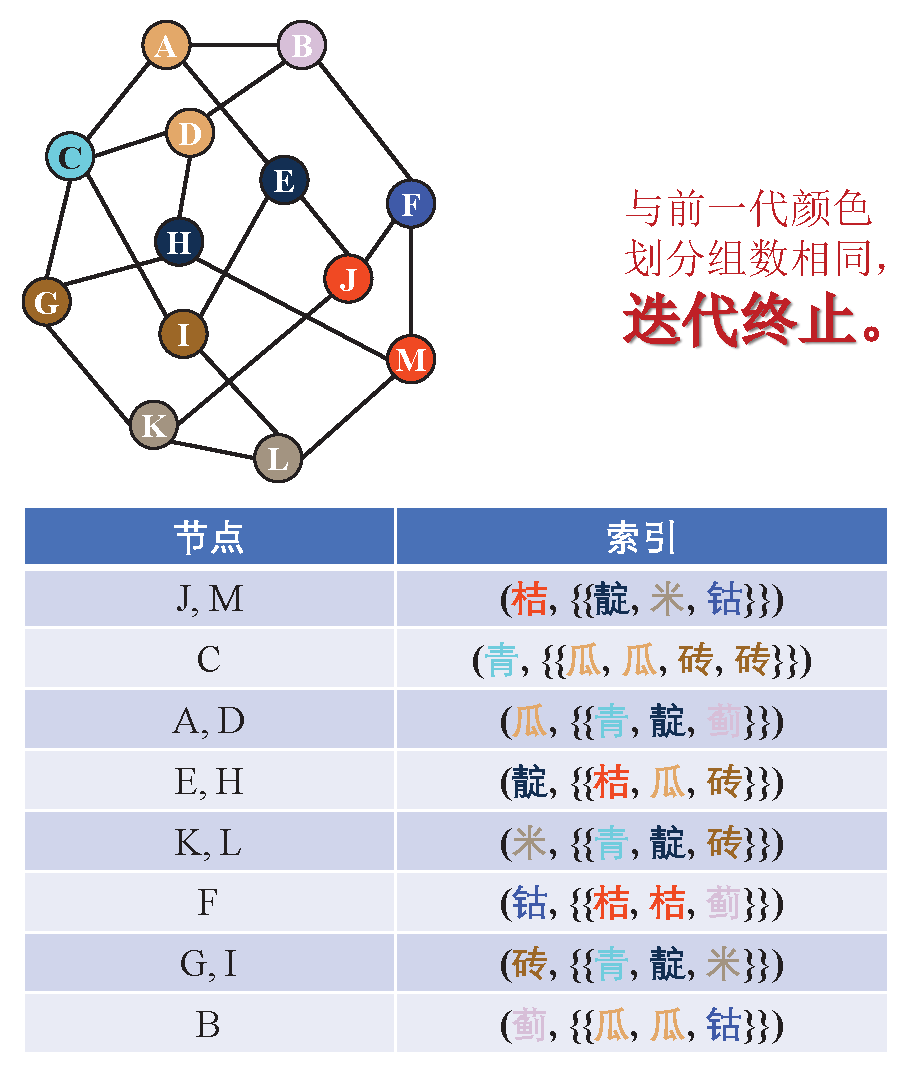
\includegraphics[scale=0.38]{pic/1wl-iter6.eps}
	\end{figure}
\end{frame}

\begin{frame}{WL测试}
	两个{\color{red}\textbf{图}}$\mathscr{G}_1$和$\mathscr{G}_2$，经过一维Weisfeiler-Lehman算法计算得到最终节点颜色，
	\begin{figure}
		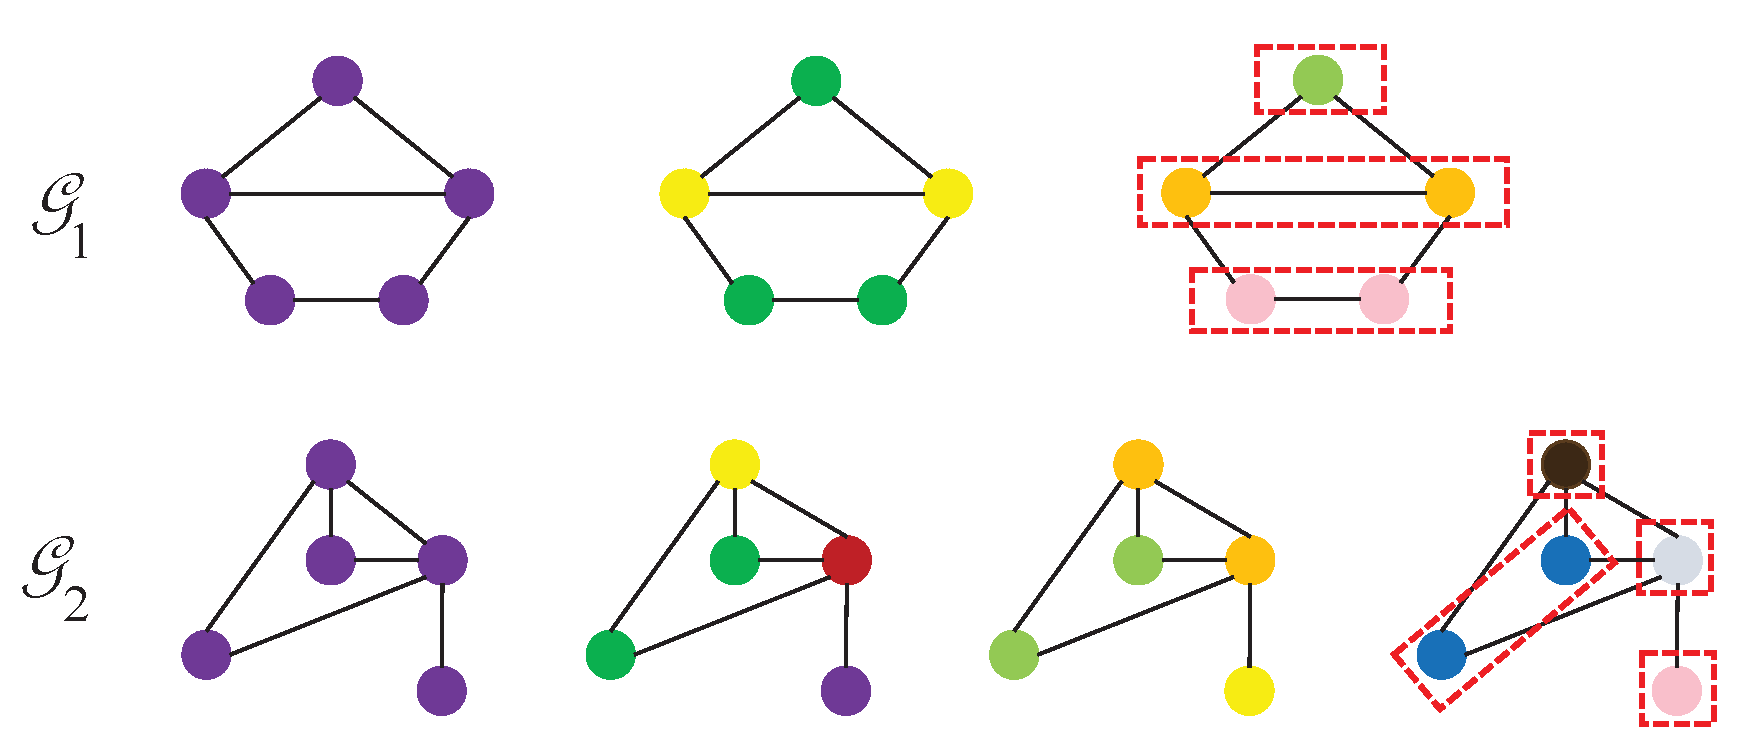
\includegraphics[scale=0.35]{pic/nonisogt.eps}
	\end{figure}
	如果最终节点颜色（标签）的{\color{red}\textbf{种类数不同}}，那么图$\mathscr{G}_1$和$\mathscr{G}_2${\color{red}\textbf{不同构}}。
\end{frame}

\begin{frame}{WL测试（逆否命题）}
	两个{\color{red}\textbf{同构的图}}$\mathscr{G}_1$和$\mathscr{G}_2$，经过一维Weisfeiler-Lehman算法计算得到最终节点颜色，
	\begin{figure}
		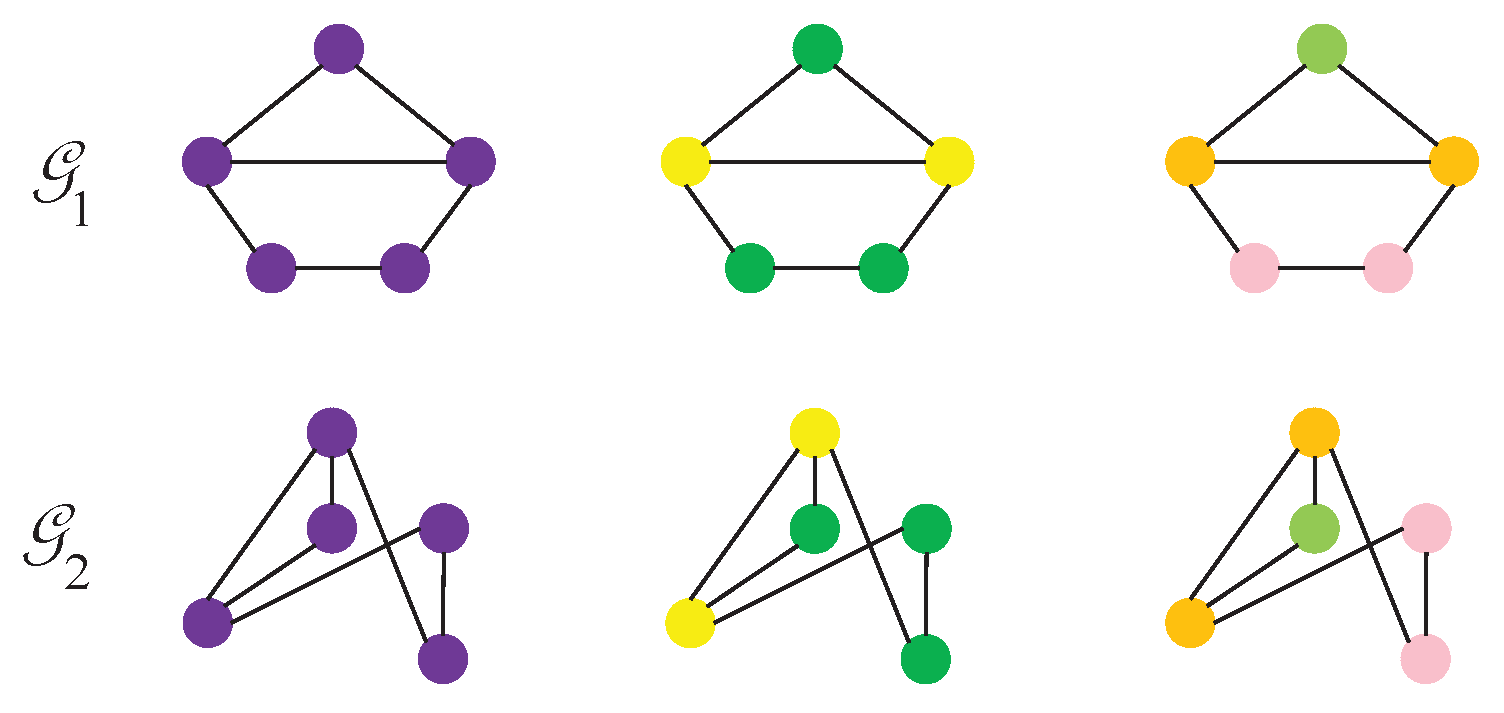
\includegraphics[scale=0.35]{pic/isogt.eps}
	\end{figure}
	最终节点颜色（标签）的{\color{red}\textbf{种类数相同}}。
\end{frame}

\begin{frame}{图神经网络与WL测试}
	\begin{formal}
		\textbf{定义}\\
		一个多重集（multiset）允许普通集合中的元素多次出现。多重集的形式化定义为一个两元组
		\begin{equation}
			X=\left(S,m\right),
		\end{equation}
		$S$为$X$的支集（underlying set），其由不可重复的元素（distinct elements）组成。$m:S\to\mathbb{N}_{\ge1}$给出每个元素的个体数目（multiplicity）。
	\end{formal}
\end{frame}

\begin{frame}{图神经网络与WL测试（续）~\cite{xu2019gin}}
	\begin{formal}
		\textbf{引理1}\\
		仍给两个不同构的图$\mathscr{G}_1$和$\mathscr{G}_2$，如果一个图神经网络$\mathcal{A}:\mathscr{G}\to\mathbb{R}^d$将$\mathscr{G}_1$和$\mathscr{G}_2$映射为{\color{red}不同的嵌入表示}，WL测试也能判断$\mathscr{G}_1$和$\mathscr{G}_2${\color{red}不同构}。
	\end{formal}
	{\color{red}假设$k$次迭代后，图神经网络$\mathcal{A}$有$\mathcal{A}\left(\mathscr{G}_1\right)\neq\mathcal{A}\left(\mathscr{G}_2\right)$，WL测试不能判断$\mathscr{G}_1$和$\mathscr{G}_2$不同构}。\\
	从而，前$k-1$代中，$\mathscr{G}_1$和$\mathscr{G}_2$在WL测试中的节点标签始终相同。\\
	特别地，$\mathscr{G}_1$和$\mathscr{G}_2$在WL测试的第$i$（$i=0\dots k-1$）代和第$i+1$代有相同的节点标签，从而$\mathscr{G}_1$和$\mathscr{G}_2$有相同的邻居节点标签多重集$\left\{\left(l_v^{\left(i\right)},\left\{l_u^{\left(i\right)}:u\in\mathcal{N}\left(v\right)\right\}\right)\right\}$。
\end{frame}

\begin{frame}{图神经网络与WL测试（续）}
	接下来需要证明：{\color{red}任意两个节点$u$和$v$，若在WL测试第$i$（$0\le i\le K$）代时的节点标签$l_u^{\left(i\right)}=l_v^{\left(i\right)}$，则必有在GNN第$i$代时的节点特征$h_u^{\left(i\right)}=h_v^{\left(i\right)}$}。\\
	当$i=0$时，结论显然成立，因为初始的节点特征（标签）矩阵相同。\\
	假设当$i=j$时，结论成立。当$i=j+1$时，若$l_u^{\left(j+1\right)}=l_v^{\left(j+1\right)}$，由前一页可知：
	\begin{equation}
		\left\{\left(l_u^{\left(j\right)},\left\{l_{u'}^{\left(j\right)}:u'\in\mathcal{N}\left(u\right)\right\}\right)\right\}=\left\{\left(l_v^{\left(j\right)},\left\{l_{v'}^{\left(j\right)}:v'\in\mathcal{N}\left(v\right)\right\}\right)\right\},
	\end{equation}
	由$i=j$时的假设可得
	\begin{equation}
		\left\{\left(h_u^{\left(j\right)},\left\{h_{u'}^{\left(j\right)}:u'\in\mathcal{N}\left(u\right)\right\}\right)\right\}=\left\{\left(h_v^{\left(j\right)},\left\{h_{v'}^{\left(j\right)}:v'\in\mathcal{N}\left(v\right)\right\}\right)\right\},
	\end{equation}
	在GNN的计算过程中，每个节点应用了同样的聚合函数（AGGREGATE）和组合函数（CONCAT/COMBINE），因而有$h_u^{\left(j+1\right)}=h_v^{\left(j+1\right)}$。
\end{frame}

\begin{frame}{图神经网络与WL测试（续）}
	由上一页中的数学归纳法，证得：{\color{red}任意两个节点$u$和$v$，若在WL测试第$i$（$0\le i\le K$）代时的节点标签$l_u^{\left(i\right)}=l_v^{\left(i\right)}$，则必有在GNN第$i$代时的节点特征$h_u^{\left(i\right)}=h_v^{\left(i\right)}$}。\\
	因此，对于任意节点$v\in\mathscr{V}$，存在一个隐式的双射$\phi$，使得$h_v^{\left(i\right)}=\phi\left(l_v^{\left(i\right)}\right)$
	\begin{equation}
		\left\{\left(h_v^{\left(i\right)},\left\{h_{v'}^{\left(i\right)}:v'\in\mathcal{N}\left(v\right)\right\}\right)\right\}=\left\{\left(\phi\left(l_v^{\left(i\right)}\right),\left\{\phi\left(l_{v'}^{\left(i\right)}\right):v'\in\mathcal{N}\left(v\right)\right\}\right)\right\},
	\end{equation}
	从而，图$\mathscr{G}_1$和$\mathscr{G}_2$在$i+1$代时有相同的GNN节点特征$\left\{h_v^{\left(i+1\right)}\right\}$多重集。由于图池化（图读出）操作是置换不变的，故有$\mathcal{A}\left(\mathscr{G}_1\right)=\mathcal{A}\left(\mathscr{G}_2\right)$，{\color{red}与假设矛盾}。
\end{frame}

\begin{frame}{设计更高效的图神经网络：GIN设计思想~\cite{xu2019gin}}
	\begin{formal}
		\textbf{定理}\\
		令$\mathcal{A}:\mathscr{G}\to\mathbb{R}^d$为一个GNN模型。在足够数量的GNN层数后，$\mathcal{A}$能将WL测试判断为不同构的两个图$\mathscr{G}_1$和$\mathscr{G}_2$映射到不同的嵌入表示 {\color{red}\textbf{if}}:
		\begin{enumerate}
			\item $\mathcal{A}$按以下公式迭代聚合和更新节点特征：
			\begin{equation}
				h_v^{\left(k\right)}=\phi\left(h_v^{\left(k-1\right)},f\left(\left\{h_u^{\left(k-1\right)}:u\in\mathcal{N}\left(v\right)\right\}\right)\right),
			\end{equation}
			其中，作用在节点特征多重集上的函数$f$、函数$\phi$是{\color{red}\textbf{单射的}}（injective）；
			\item 作用在节点特征多重集上的$\mathcal{A}$的图读出也是{\color{red}\textbf{单射的}}。
		\end{enumerate}
	\end{formal}
\end{frame}

\begin{frame}{设计更高效的图神经网络：GIN设计思想（续）}
	由于图读出函数是单射的，故而其将不同的节点特征多重集映射到不同的嵌入表示。接下来需要看$\mathcal{A}$的聚合过程。\\
	WL测试使用了一个单射$g$来更新节点标签$l_v^{\left(k\right)}$
	\begin{equation}
		l_v^{\left(k\right)}=g\left(l_v^{\left(k-1\right)},\left\{l_u^{\left(k\right)}:u\in\mathcal{N}\left(v\right)\right\}\right).
	\end{equation}
	因而，一种证明思路为证明：{\color{red}对任意第$k$代，总存在一个单射$\varphi$，使得$h_v^{\left(k\right)}=\varphi\left(l_v^{\left(k\right)}\right)$}。\\
	$k=0$时，显然成立。由于$h_v^{\left(0\right)}=l_v^{\left(0\right)}$，$\varphi$为恒等变换。\\
	假设$k-1$代时结论成立，则
	\begin{equation}
		h_v^{\left(k\right)}=\phi\left(\varphi\left(l_v^{\left(k-1\right)}\right),f\left(\left\{\varphi\left(l_u^{\left(k-1\right)}\right):u\in\mathcal{N}\left(v\right)\right\}\right)\right).
	\end{equation}
\end{frame}

\begin{frame}{设计更高效的图神经网络：GIN设计思想（续）}
	由于单射的嵌套也是单射的，故应存在单射$\psi$使得
	\begin{equation}
		h_v^{\left(k\right)}=\psi\left(l_v^{\left(k-1\right)},\left\{l_u^{\left(k-1\right)}:u\in\mathcal{N}\left(v\right)\right\}\right).
	\end{equation}
	从而
	\begin{equation}
		h_v^{\left(k\right)}=\psi\circ g^{-1}\circ g\left(l_v^{\left(k-1\right)},\left\{l_u^{\left(k-1\right)}:u\in\mathcal{N}\left(v\right)\right\}\right)=\psi\circ g^{-1}\left(l_v^{\left(k\right)}\right),
	\end{equation}
	$\psi\circ g^{-1}$是单射的，故而存在单射$\varphi=\psi\circ g^{-1}$使得$h_v^{\left(k\right)}=\varphi\left(l_v^{\left(k\right)}\right)$。
\end{frame}

\begin{frame}{设计更高效的图神经网络：GIN设计思想（续）}
	\begin{formal}
		\textbf{引理2}\\
		假设输入特征空间$\mathcal{X}$是可数的（countable）。令$g^{\left(k\right)}$为GNN第$k$（$k=1\dots\L$）层计算的参数构成的函数，$g^{\left(1\right)}$定义为有限大小（bounded size）的多重集$X\subset\mathcal{X}$。$g^{\left(k\right)}$（节点隐含层特征$h_v^{\left(k\right)}$）的范围是可数的。
	\end{formal}
	\begin{formal}
		\textbf{引理3}\\
		假设$\mathcal{X}$是可数的。存在函数$f:\mathcal{X}\to\mathbb{R}^n$，使得对于每个有限大小的多重集$X\subset\mathcal{X}$，$h\left(X\right)=\sum\limits_{x\in X}f\left(x\right)$是unique的。另外，任意应用在多重集上的函数$g$可以分解为$g\left(X\right)=\phi\left(\sum\limits_{x\in X}f\left(x\right)\right)$。
	\end{formal}
\end{frame}

\begin{frame}{设计更高效的图神经网络：GIN设计思想（续）}
	\begin{formal}
		\textbf{推论}\\
		假设$\mathcal{X}$是可数的，存在函数$f:\mathcal{X}\to\mathbb{R}^n$，使得对于$\epsilon$无限多种选择（包含所有不合理的数值），对每个有限大小的多重集$\left(c,X\right)$（$c\in\mathcal{X}$、$X\subset\mathcal{X}$），$h\left(c,X\right)=\left(1+\epsilon\right)\cdot f\left(c\right)+\sum\limits_{x\in X}f\left(x\right)$是unique的。另外，任意应用在多重集上的函数$g$可以分解为$g\left(c,X\right)=\varphi\left(\left(1+\epsilon\right)\cdot f\left(c\right)+\sum\limits_{x\in X}f\left(x\right)\right)$
	\end{formal}
	可以使用多层感知机（multi-layer perceptrons，MLPs）建模学习推论中的函数$f$和$g$，$f^{\left(k+1\right)}\circ g^{\left(k\right)}$建模为建模为一层MLP。将$\epsilon$设置为可学习的参数或者为固定的参数，
	\begin{equation}
		h_v^{\left(k\right)}=MLP^{\left(k\right)}\left(\left(1+\epsilon^{\left(k\right)}\right)\cdot h_v^{\left(k-1\right)}+\sum\limits_{u\in\mathcal{N}\left(v\right)}h_u^{\left(k-1\right)}\right)
	\end{equation}
\end{frame}

\begin{frame}{设计更高效的图神经网络：GIN设计思想（续）}
	节点的特征随着迭代次数的增加，会变得更加精炼（refined）和全局（global）。更早迭代次数（earlier iterations）的节点特征有时能泛化效果更好（generalize better）。为考虑结构性信息，GIN使用利用了所有深度/迭代次数进行推理：
	\begin{equation}
		h_G=\text{CONCAT}\left(\text{READOUT}\left(\left\{h_v^{\left(k\right)}|\,k=0\dots K\right\}\right)\right).
	\end{equation}
\end{frame}



\section{类比热传导}


\begin{frame}{一维空间中的热传导~\cite{wiki2024heat}}
	给定一个放置在\textbf{X轴}上{\color{red}均匀材质}的{\color{red}细杆}（thin rod），其横截面积为$A$。
	\begin{figure}
		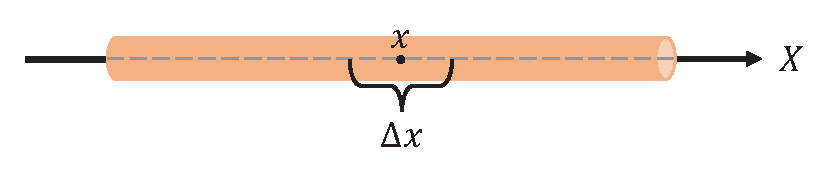
\includegraphics[scale=0.5]{pic/rod.eps}
	\end{figure}
	\begin{formal}
		{\color{red}\textbf{温度（temperature）}}是关于位置和时间的函数，记作$u$，$u\left(x,t\right)$表示$t$时刻位置$x$处的温度。 \\
		{\color{red}\textbf{热流量（heat flow）}}也是关于位置和时间的函数，记为$\varPhi$，$\varPhi\left(x,t\right)$表示$t$时刻位置$x$处沿\textbf{X轴}正方向的热流量。\\
		{\color{red}\textbf{热能（heat energy）}}也是关于位置和时间的函数，记为$Q$，$Q\left(x,t\right)$表示$t$时刻位置$x$处单位体积上的热能。
	\end{formal}
\end{frame}

\begin{frame}{一维空间中的热传导（续）}
	\begin{figure}
		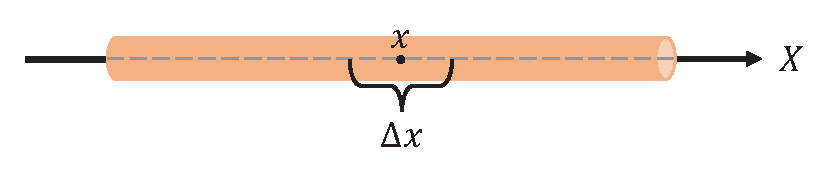
\includegraphics[scale=0.5]{pic/rod.eps}
	\end{figure}
	\begin{formal}
		{\color{red}\textbf{傅里叶定律（Fourier's law）}} \\
		在导热现象中，单位时间内通过给定截面的热量，正比例于垂直于该截面方向上的温度变化率和截面面积，而热量传递的方向则与温度升高的方向相反。
		\begin{equation}
			\label{eq:heatflow}
			\varPhi=-\lambda\frac{\partial u}{\partial x}A,
		\end{equation}
		$\lambda$为材料的\textbf{热导度}（或称导热系数）（thermal conductivity）\footnote{在稳定传热条件下，两侧温差为1K的厚度为1m的材料，在1s内，通过1$\text{m}^2$截面传递的热量。}。
	\end{formal}
\end{frame}

\begin{frame}{一维空间中的热传导（续）}
	\begin{figure}
		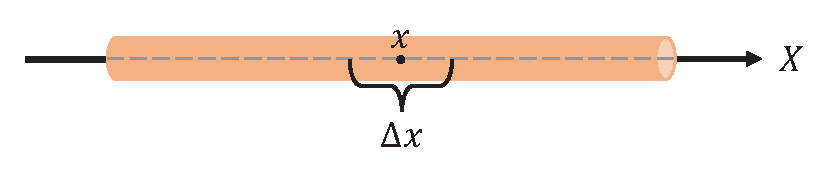
\includegraphics[scale=0.5]{pic/rod.eps}
	\end{figure}
	\begin{formal}
		参考初中物理学知识，{\color{red}\textbf{以坐标值$x$为中心的足够小的一段长度$\Delta x$上的热能随时间的变化率}}可计算如下：
		\begin{equation}
			\label{eq:heateng}
			\frac{\partial Q}{\partial t}=c\rho A\frac{\partial u}{\partial t},
		\end{equation}
		$c$为材料的\textbf{比热容}（specific heat capacity），$\rho$为材料的\textbf{密度}（density）。
	\end{formal}
\end{frame}

\begin{frame}{一维空间中的热传导（续）}
	\begin{figure}
		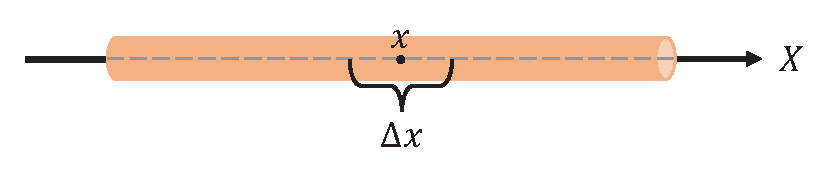
\includegraphics[scale=0.5]{pic/rod.eps}
	\end{figure}
	\begin{formal}
		根据{\color{red}\textbf{能量守恒定律（law of conservation of energy）}}，在$\Delta x$上存储的热能的变化率与热能传递速率（热流量的梯度）{\color{red}\textbf{相等}}，即
		\begin{equation}
			\frac{\partial Q}{\partial t}=-\frac{\partial\varPhi}{\partial x}.
		\end{equation}\\
		联立公式\ref{eq:heatflow}、公式\ref{eq:heateng}和上式，有
		\begin{equation}
			\label{eq:ns1dhc}
			\frac{\partial u}{\partial t}=-\frac{1}{c\rho}\frac{\partial\varPhi}{\partial x}\frac{1}{A}=-\frac{1}{c\rho}\frac{\partial}{\partial x}\left(-\lambda\frac{\partial u}{\partial x}A\right)\frac{1}{A}=\frac{\lambda}{c\rho}\frac{\partial^2 u}{\partial x^2}
		\end{equation}
	\end{formal}
\end{frame}

\begin{frame}{一维空间中的热传导（续）}
	\begin{formal}
		记$\alpha=\frac{\lambda}{c\rho}$，$\alpha$为常数，称为材料的\textbf{热扩散率}（thermal diffusivity）。
		则公式\ref{eq:ns1dhc}简写为
		\begin{equation}
			\frac{\partial u}{\partial t}=\alpha\frac{\partial^2 u}{\partial x^2},
		\end{equation}
		即{\color{red}\textbf{一维空间中的热传导公式}}。\\
		等式右侧可改写成{\color{red}\textbf{差分形式}}，记$i-1,i,i+1$为\textbf{X轴}上三个间隔足够小的坐标点，有
		\begin{equation}
			\label{eq:dis1dhc}
			\frac{\partial u_i}{\partial t}=\alpha\left(\left(u_{i+1}-u_i\right)-\left(u_i-u_{i-1}\right)\right),
		\end{equation}
		上式中，$u\left(i,\tau\right)$（$\tau$表示任意时刻）简记为$u_i$。
	\end{formal}
\end{frame}

\begin{frame}{高维欧式空间中的热传导}
	\begin{formal}
		在高维空间中，{\color{red}\textbf{拉普拉斯算子（Laplacian operator）}}定义为各个方向上二阶偏导数之和，即
		\begin{equation}
			\Delta u=\sum\limits_{i=1}^N\frac{\partial^2u}{\partial x_i^2}.
		\end{equation}
	\end{formal}
	\begin{formal}
		于是，{\color{red}\textbf{高维欧式空间中的热传导公式}}为
		\begin{equation}
			\frac{\partial u}{\partial t}=\alpha\Delta u.
		\end{equation}
	\end{formal}
\end{frame}

\begin{frame}{图上的热传导}
	在一维空间中，\textbf{X轴}上的{\color{red}\textbf{坐标点$i$只与左右相邻的两个坐标点$i-1$和$i+1$之间发生热传递}}。类似地，在\textbf{图$\mathscr{G}$}中，设定{\color{red}\textbf{节点$i$只与其邻居节点$j\in\mathcal{N}_i$之间发生热传递}}。
	
	给定一个节点$i$，参考公式\ref{eq:dis1dhc}，有
	\begin{equation}
		\label{eq:tcgraph}
		\frac{\partial u_i}{\partial t}=\alpha\sum\limits_{j\in\mathcal{N}_i}\left(u_j-u_i\right)=\alpha\sum\limits_j\textbf{A}_{ij}\left(u_j-u_i\right).
	\end{equation}
	结合乘法分配律，
	\begin{equation}
		\label{eq:shcg}
		\begin{aligned}
			\frac{\partial u_i}{\partial t}&=\alpha\sum\limits_j\textbf{A}_{ij}\left(u_j-u_i\right)
			=-\alpha\left(u_i\sum\limits_j\textbf{A}_{ij}-\sum\limits_j\textbf{A}_{ij}u_j\right)\\
			&=-\alpha\left(\textbf{D}_{ii}u_i-\sum\limits_j\textbf{A}_{ij}u_j\right).
		\end{aligned}
	\end{equation}
\end{frame}

\begin{frame}{图上的热传导（续）}
	参考公式\ref{eq:shcg}，将所有节点的热传递计算公式排成列，有
	\begin{equation}
		\begin{bmatrix}
			\frac{\partial u_1}{\partial t} \\ \frac{\partial u_2}{\partial t} \\ \cdots \\ \frac{\partial u_{\left|\mathscr{V}\right|}}{\partial t}
		\end{bmatrix}
		=-\alpha\left(
		\begin{bmatrix}
			\textbf{D}_{11}\times u_1 \\ \textbf{D}_{22}\times u_2 \\ \cdots \\ \textbf{D}_{\left|\mathscr{V}\right|\left|\mathscr{V}\right|}\times u_{\left|\mathscr{V}\right|}
		\end{bmatrix} - \textbf{A}
		\begin{bmatrix}
			u_1 \\ u_2 \\ \cdots \\ u_{\left|\mathscr{V}\right|}
		\end{bmatrix}\right).
	\end{equation}
	记$\vec{\textbf{u}}=\left[u_1,u_2,\dots,u_{\left|\mathscr{V}\right|}\right]^\top$，有
	\begin{equation}
		\frac{\partial \vec{\textbf{u}}}{\partial t}=-\alpha\left(\textbf{D}-\textbf{A}\right)\vec{\textbf{u}},
	\end{equation}
\end{frame}

\begin{frame}{图上的热传导（续）}
	\begin{formal}
		$\textbf{D}-\textbf{A}$称为图的{\color{red}\textbf{拉普拉斯矩阵（Laplacian matrix）}}，记为$\textbf{L}$，则{\color{red}\textbf{图上的热传导公式}}为
		\begin{equation}
			\frac{\partial \vec{\textbf{u}}}{\partial t}=-\alpha\textbf{L}\vec{\textbf{u}}.
		\end{equation}
		回顾{\color{red}\textbf{欧式空间中的热传导公式}}
		\begin{equation*}
			\frac{\partial u}{\partial t}=\alpha\Delta u.
		\end{equation*}
	\end{formal}
	{\color{red}二者具有一样的形式！}\textbf{GNN的实质}：图上特征和消息中的流动和传播。这个传播最原始的形态就是状态的变化正比于图空间中拉普拉斯算子作用在当前的状态~\cite{jr2019gcn}。
\end{frame}

\begin{frame}{图上的热传导（续）}
	参考公式\ref{eq:tcgraph}
	\begin{equation*}
		\frac{\partial u_i}{\partial t}=\alpha\sum\limits_j\textbf{A}_{ij}\left(u_j-u_i\right).
	\end{equation*}
	在时域上离散上式
	\begin{equation}
		\begin{aligned}
			\vec{\textbf{u}}_i^{\left(t+1\right)}&=\vec{\textbf{u}}_i^{\left(t\right)}+\alpha\sum\limits_j\textbf{A}_{ij}\left(\vec{\textbf{u}}_j^{\left(t\right)}-\vec{\textbf{u}}_i^{\left(t\right)}\right) \\
			&=\left(1-\alpha\textbf{D}_{ii}\right)\vec{\textbf{u}}_i^{\left(t\right)}+\alpha\sum\limits_j\textbf{A}_{ij}\vec{\textbf{u}}_j^{\left(t\right)} \\
			&=\left(1-\alpha\textbf{D}_{ii}\right)\vec{\textbf{u}}_i^{\left(t\right)}+\alpha\sum\limits_{j\in\mathcal{N}\left(i\right)}\vec{\textbf{u}}_j^{\left(t\right)}
		\end{aligned}
	\end{equation}
	与GraphSAGE的算法核心过程{\color{red}如出一辙}！
\end{frame}



\section{参考文献}

\begin{frame}[allowframebreaks]{参考文献}
	\bibliography{ref}
	\bibliographystyle{ieeetr}
\end{frame}



\backmatter
\end{document}
